% ============================================================
%  Constraint, Trajectory, and Irreversibility:
%  A Unified Framework Across Language, Computation, and Physics
%  Author: Flyxion
%  Compiler: LuaLaTeX
% ============================================================

\documentclass[12pt, twoside]{article}

% ---- Font & Unicode ----------------------------------------
\usepackage{fontspec}
\setmainfont{texgyrepagella}[
  Extension      = .otf,
  UprightFont    = *-regular,
  BoldFont       = *-bold,
  ItalicFont     = *-italic,
  BoldItalicFont = *-bolditalic,
  Ligatures      = TeX,
  Numbers        = OldStyle
]
\usepackage{microtype}

% ---- Mathematics -------------------------------------------
\usepackage{amsmath, amsthm, amssymb, mathtools}
\usepackage{unicode-math}
\setmathfont{latinmodern-math.otf}

% ---- Layout ------------------------------------------------
\usepackage[
  a4paper,
  top=3cm, bottom=3.2cm,
  inner=3.2cm, outer=2.6cm,
  marginparwidth=2cm,
  headheight=14pt
]{geometry}

\usepackage{fancyhdr}
\pagestyle{fancy}
\fancyhf{}
\fancyhead[LE]{\small\itshape Flyxion}
\fancyhead[RO]{\small\itshape Constraint, Trajectory, and Irreversibility}
\fancyfoot[C]{\small\thepage}
\renewcommand{\headrulewidth}{0.3pt}

% ---- Sectioning --------------------------------------------
\usepackage{titlesec}
\titleformat{\section}[block]
  {\large\bfseries}{\thesection.}{0.6em}{}
\titleformat{\subsection}[block]
  {\normalsize\bfseries\itshape}{\thesubsection}{0.6em}{}
\titleformat{\subsubsection}[runin]
  {\normalsize\itshape}{\thesubsubsection}{0.5em}{}[.\enspace]

% ---- Theorem environments ----------------------------------
\theoremstyle{plain}
\newtheorem{theorem}{Theorem}[section]
\newtheorem{lemma}[theorem]{Lemma}
\newtheorem{proposition}[theorem]{Proposition}
\newtheorem{corollary}[theorem]{Corollary}

\theoremstyle{definition}
\newtheorem{definition}[theorem]{Definition}
\newtheorem{axiom}[theorem]{Axiom}
\newtheorem{example}[theorem]{Example}

\theoremstyle{remark}
\newtheorem{remark}[theorem]{Remark}
\newtheorem{notation}[theorem]{Notation}

% ---- Typography --------------------------------------------
\usepackage{setspace}
\setstretch{1.18}
\usepackage{parskip}
\setlength{\parskip}{0.55em}
\setlength{\parindent}{1.6em}

% ---- TikZ --------------------------------------------------
\usepackage{tikz}
\usetikzlibrary{arrows.meta, positioning, decorations.pathreplacing, calc}

% ---- Miscellaneous -----------------------------------------
\usepackage{xcolor}
\definecolor{deepblue}{RGB}{20,40,80}
\usepackage{epigraph}
\setlength{\epigraphwidth}{0.62\textwidth}
\renewcommand{\epigraphflush}{center}
\usepackage{enumitem}
\setlist[itemize]{noitemsep, topsep=0.3em}
\usepackage{booktabs}
\usepackage{hyperref}
\hypersetup{
  colorlinks=true,
  linkcolor=deepblue,
  urlcolor=deepblue,
  pdfauthor={Flyxion},
  pdftitle={Constraint, Trajectory, and Irreversibility}
}

% ---- Custom commands ---------------------------------------
\newcommand{\R}{\mathbb{R}}
\newcommand{\N}{\mathbb{N}}
\newcommand{\Cfg}{\mathcal{C}}
\newcommand{\Hist}{\mathcal{H}}
\newcommand{\Trans}{\mathcal{T}}
\newcommand{\Proj}{\Pi}
\newcommand{\Cone}[1]{\mathbf{C}(#1)}
\newcommand{\KES}{\mathrm{KES}}
\DeclareMathOperator{\Ent}{Ent}
\DeclareMathOperator{\rank}{rank}
\DeclareMathOperator{\supp}{supp}

% ============================================================
\begin{document}

% ---- Title page --------------------------------------------
\begin{titlepage}
\centering
\vspace*{4cm}
{\fontsize{22}{28}\selectfont\bfseries
  Constraint, Trajectory, and Irreversibility\par}
\vspace{1.2em}
{\large\itshape A Unified Framework Across Language, Computation, and Physics\par}
\vspace{3em}
{\large Flyxion\par}
\vspace{1em}
{\small Independent Researcher\par}
\vfill
{\small\itshape \today\par}
\end{titlepage}

\newpage

% ---- Abstract ----------------------------------------------
\begin{abstract}
\noindent
This essay presents a unified theoretical framework whose four invariants —
constraint primacy, irreversibility, trajectory-dependence, and projection loss —
recur identically across language, computation, artificial intelligence,
and physical cosmology.
The diversity of domains in which this framework appears is not divergence
but projection: each domain instantiates the same underlying structure
through a different representational lens, and each loses a predictable
class of properties in doing so.
After establishing the invariants formally and deriving their consequences,
the essay surveys how they manifest as generative principles across four
domain families, with particular attention to the failure modes produced
when they are violated — Goodhart drift, identity collapse, instability
under compression, and adversarial behavior — and concludes with a
methodology for reading systems that are themselves trajectory-based
and therefore resist summary.
\end{abstract}

\tableofcontents
\newpage

% ============================================================
\section*{Preface: What This Is (and Is Not)}
\addcontentsline{toc}{section}{Preface}
% ============================================================

\epigraph{\itshape
  A map is not the territory, but neither is the territory its own description.
  What is lost in the map is recoverable only by walking.}{}

This is not a portfolio.
It is not a collection of loosely related intellectual experiments assembled
after the fact under a unifying label.
It is a single system — one whose internal structure is sufficiently rich
that it must be expressed across multiple domains in order to be expressed
at all, and whose unity is therefore visible only to a reader willing to
move between those domains without collapsing them into one another.

The reader who approaches this work expecting a linear argument will find
something stranger: a set of constraints that generate trajectories,
trajectories that accumulate into histories, and histories whose structure
persists even under radical changes of medium.
Language, computation, physics, and cognition are not the subjects of this
work so much as they are its projections.
Each projection is faithful within its own register.
Each loses something that the others retain.

This creates a methodological demand.
No single section of this essay is self-sufficient.
The formal invariants of Section~2 are necessary to understand
what Section~4 is claiming when it maps them onto symbolic systems and
event calculi.
The failure modes of Section~5 are not illustrations of an abstract
principle but structural consequences that become legible only once the
invariants are in place.
The reader is therefore not expected to consume the work sequentially,
but to navigate it — to recognize which projection they are currently
reading and to locate that projection within the larger structure.

One further preliminary.
The apparent fragmentation of the larger research program from which this
essay emerges — its distribution across formal monographs, computational
implementations, game prototypes, and theoretical essays — is not a
feature of disorganization.
It is a consequence of the framework itself.
A theory of irreversibility and trajectory-dependence cannot be adequately
expressed in a single stable artifact.
It must be reconstructed by the reader from its projections,
exactly as a wave function is reconstructed from its measurements,
or a historical identity from the paths that generated it.

This essay is one projection.
It is not the whole.

\newpage

% ============================================================
\section{The Core Problem}
% ============================================================

Contemporary modeling practice across the sciences, engineering,
and the design of intelligent systems shares a characteristic error:
it treats states as primary and processes as derivative.
A system is described by where it is, not by how it got there.
Its future is predicted from its present configuration, not from the
structured history of transitions that produced that configuration.
And its evaluation is conducted by measuring scalar quantities
— performance metrics, objective functions, loss values, utility scores —
that stand in for the system's relationship to its environment
without preserving the structure of that relationship.

This error is not merely technical.
It is ontological.
It assigns the wrong category of entity — static configurations and scalar
values — the role that belongs to processes, trajectories, and constraint
structures.
The consequences ramify through every domain in which such modeling is
applied, and they are predictable.
When a system's identity is modeled as its current state,
that identity becomes fragile: any perturbation that moves the state
vector displaces the identity, even if the generative process that
produced the state is intact.
When a system's behavior is modeled as optimization of a scalar objective,
the system learns to maximize the proxy at the expense of the underlying
structure the proxy was intended to represent — a phenomenon now
sufficiently general to constitute a theorem.
When a system's history is compressed into a summary statistic,
the information discarded by that compression generates systematic
downstream errors that no amount of fine-tuning of the retained
representation can recover.

These three failure modes — fragility under perturbation,
proxy maximization, and compression error — are not independent.
They are consequences of the same underlying mistake: the replacement
of trajectory-based, constraint-structured descriptions by state-based,
objective-structured ones.

The present framework does not attempt to patch this mistake within
the existing paradigm.
It proposes an alternative foundation, one in which constraints are primary,
trajectories are the basic objects of analysis, irreversibility is not a
defect to be managed but a constitutive feature of identity and meaning,
and projection loss is a formal property to be characterized rather than
a nuisance to be minimized.

Before developing the framework formally, it is worth noting what makes
this approach non-trivial.
The claim is not merely that process matters as well as state, or that
history should be taken into account as an additional variable.
The claim is that the very category of state is a derived, secondary
concept — useful, but dependent on a prior account of what constraints
and transitions are available in the system.
A state, in the framework to be developed, is a configuration admissible
under a constraint structure at a moment in a trajectory.
It has no meaning apart from that context.
This is a stronger claim than the usual injunction to be historically
sensitive, and it has formal consequences that will be developed in
the sections that follow.

The fragmentation of contemporary intellectual and technological practice
also calls for comment.
Physics, linguistics, computer science, and the study of cognition have
developed largely independent technical vocabularies, independent formal
tools, and independent bodies of intuition.
This is in many respects productive: specialized tools are more powerful
than general ones within their domain of application.
But it means that shared structure is routinely missed.
The constraint structures that govern syntactic possibility in a
natural language are formally homomorphic to the constraint structures
that govern computationally admissible paths in an event calculus.
The projection loss incurred when a physical field is discretized on a
lattice is formally identical in structure to the projection loss incurred
when a semantic trajectory is compressed into a summary embedding.
These homomorphisms are not metaphors.
They are the subject matter of this essay.

\newpage

% ============================================================
\section{The Invariants}
% ============================================================

\epigraph{\itshape
  It is not the destination that determines the traveler's identity,
  but the set of paths that were and were not taken to reach it.}{}

This section develops the four invariants of the framework with
full formal precision.
The invariants are not axioms in the logician's sense — they are not
adopted without argument.
They are propositions for which motivation is given and from which
consequences are derived.
However, within the framework they function as load-bearing assumptions:
everything that follows depends on them, and the framework is to be
evaluated by the fertility and accuracy of those consequences.

% ------------------------------------------------------------
\subsection{Constraint Primacy}
% ------------------------------------------------------------

The first invariant concerns the ontological order between constraints
and objectives.
Standard optimization-based modeling places objectives first:
a system is defined by what it is trying to achieve,
and constraints are the obstacles or guardrails placed around that
achievement.
This ordering is reversed here.

\begin{definition}[Constraint Structure]
A \emph{constraint structure} is a triple $(\Cfg, \Trans, \mathcal{F})$
where $\Cfg$ is a set of configurations, $\Trans \subseteq \Cfg \times \Cfg$
is the set of admissible transitions, and $\mathcal{F} \subseteq 2^{\Cfg}$
is a filter specifying which subsets of $\Cfg$ constitute admissible
initial conditions.
\end{definition}

\begin{definition}[Admissible Path]
Given a constraint structure $(\Cfg, \Trans, \mathcal{F})$, an
\emph{admissible path} of length $n$ is a sequence
$\gamma = (c_0, c_1, \ldots, c_n)$ with $c_0 \in \bigcup \mathcal{F}$
and $(c_i, c_{i+1}) \in \Trans$ for all $0 \leq i < n$.
The set of all admissible paths is denoted $\mathrm{Path}(\Cfg, \Trans, \mathcal{F})$.
\end{definition}

The fundamental claim of constraint primacy is that a system is \emph{defined}
by its constraint structure — that the constraint structure is explanatorily
and ontologically prior to any objective function that might be imposed
upon it.

\begin{axiom}[Constraint Primacy]
\label{ax:constraint}
For any system $S$, there exists a constraint structure
$\mathcal{K}(S) = (\Cfg_S, \Trans_S, \mathcal{F}_S)$ such that every
behavioral property of $S$ is a property of
$\mathrm{Path}(\mathcal{K}(S))$.
Objective functions on $S$ are real-valued functions on
$\mathrm{Path}(\mathcal{K}(S))$; they presuppose the constraint
structure and cannot replace it.
\end{axiom}

The practical consequence of Axiom~\ref{ax:constraint} is that
optimization-based descriptions of a system are necessarily incomplete.
An objective function selects among admissible paths; it does not
generate the space of admissible paths, and it cannot recover
that space once it has been collapsed.
A system specified only by its objective function, with no account of
its constraint structure, is underspecified in the most fundamental sense:
its possible behaviors are not determined.

\begin{remark}
Note that constraint primacy does not prohibit the use of objective
functions.
It prohibits treating them as foundational.
An objective function that tracks a genuine property of the system's
admissible paths is a useful analytical tool.
An objective function adopted as a proxy for an incompletely understood
constraint structure — which is the typical case in machine learning and
institutional design — is a source of predictable failure.
\end{remark}

% ------------------------------------------------------------
\subsection{Irreversibility}
% ------------------------------------------------------------

The second invariant concerns the directionality of time in any
system with non-trivial constraint structure.

\begin{definition}[Reversible and Irreversible Transitions]
A transition $(c, c') \in \Trans$ is \emph{reversible} if
$(c', c) \in \Trans$; it is \emph{irreversible} otherwise.
A constraint structure is \emph{irreversible} if it contains at least
one irreversible transition.
\end{definition}

Every system of interest in the domains surveyed by this essay —
physical systems evolving under thermodynamic constraints,
computational systems executing programs, linguistic systems producing
utterances, cognitive systems acquiring concepts — is irreversible
in this sense.
This is not a special feature of any one domain; it is a consequence of
the second law of thermodynamics at the physical level
and of the computational irreducibility of execution histories
at the computational level.

\begin{definition}[History and Path-Identity]
The \emph{history} of a system $S$ up to time $t$ is the admissible
path $\gamma_t = (c_0, c_1, \ldots, c_t)$ that produced the current
configuration $c_t$.
Two configurations $c$ and $c'$ are \emph{path-distinct} even if $c = c'$
whenever their generating histories differ:
$\gamma_t \neq \gamma'_t$.
The \emph{identity} of a system at time $t$ is its history $\gamma_t$,
not its current configuration $c_t$.
\end{definition}

This definition has a counterintuitive consequence that is worth
making explicit.

\begin{theorem}[Identity is Path-Dependent]
\label{thm:identity}
Let $S$ and $S'$ be two systems with identical current configurations
$c_t = c'_t$ but distinct histories $\gamma_t \neq \gamma'_t$.
Then $S$ and $S'$ are distinct systems, and no property of $S$
that depends on its history is predictable from $c_t$ alone.
\end{theorem}

\begin{proof}
By definition, the identity of a system is its history.
If $\gamma_t \neq \gamma'_t$, the identities are distinct.
Any property $P$ of $S$ that is a function of $\gamma_t$ takes the form
$P(S) = f(\gamma_t)$ for some function $f$.
Since $\gamma_t \neq \gamma'_t$ and $f$ is evaluated on the history,
$f(\gamma_t)$ and $f(\gamma'_t)$ are in general distinct,
and neither is determined by $c_t = c'_t$ alone.
\end{proof}

The import of Theorem~\ref{thm:identity} is immediate for any practice
that attempts to predict, evaluate, or control systems from their
current state.
Such prediction is reliable only for properties that are functions of
the current configuration alone — a severely restricted class.
For behavioral, semantic, and dispositional properties,
the history is indispensable.

\begin{axiom}[Irreversibility]
\label{ax:irrev}
For any system $S$ with non-trivial constraint structure,
the identity of $S$ is its history $\gamma_t$,
not its current configuration $c_t$.
The map $\gamma_t \mapsto c_t$ is in general many-to-one and
cannot be inverted without additional information.
\end{axiom}

% ------------------------------------------------------------
\subsection{Trajectory-Dependence}
% ------------------------------------------------------------

The third invariant extends irreversibility from identity to meaning.
If identity is path-dependent, then so too must be any property
that depends on identity — in particular, semantic properties:
what a symbol means, what a computation signifies, what a physical
quantity represents.

\begin{definition}[Semantic Function]
A \emph{semantic function} on a constraint structure
$(\Cfg, \Trans, \mathcal{F})$ is a function
$\sigma: \mathrm{Path}(\Cfg, \Trans, \mathcal{F}) \to M$
where $M$ is a meaning space (a structured set appropriate to the domain).
A semantic function is \emph{state-reducible} if there exists a function
$\hat{\sigma}: \Cfg \to M$ such that
$\sigma(\gamma) = \hat{\sigma}(\gamma_{|\gamma|})$
for all admissible paths $\gamma$,
where $\gamma_{|\gamma|}$ denotes the terminal configuration.
\end{definition}

\begin{theorem}[Non-Reducibility of Semantic Functions]
\label{thm:semantic}
In any irreversible constraint structure, there exist semantic functions
that are not state-reducible.
\end{theorem}

\begin{proof}
Let $(c, c') \in \Trans$ be irreversible, and let $\gamma$ and $\gamma'$
be two admissible paths with $\gamma_{|\gamma|} = \gamma'_{|\gamma'|} = c'$
but $\gamma \neq \gamma'$ (which is possible since the transition is
irreversible and paths to $c'$ need not be unique).
Define $\sigma$ by: $\sigma(\gamma) = 0$ and $\sigma(\gamma') = 1$
for all paths terminating at $c'$ via these respective routes,
and extend consistently elsewhere.
Then $\sigma$ is a well-defined semantic function, but for any candidate
$\hat{\sigma}$, $\hat{\sigma}(c') = \sigma(\gamma) = 0$
requires $\sigma(\gamma') = 0$, a contradiction.
Hence no state-reducible $\hat{\sigma}$ represents $\sigma$.
\end{proof}

The philosophical interpretation of Theorem~\ref{thm:semantic}
is that meaning — in the broadest sense that includes physical significance,
computational semantics, and linguistic reference — is irreducibly
path-dependent in any system with non-trivial irreversibility.
The meaning of a symbol is not a function of its current form
but of the trajectory of transformations through which it arrived
at that form and was used.
The meaning of a computation is not its output but the history of
state transitions that produced it.

\begin{axiom}[Trajectory-Dependence]
\label{ax:traj}
Meaning, reference, and semantic content are functions of admissible paths,
not of terminal configurations.
Any representation that compresses a trajectory to a state
discards semantic information that cannot be recovered from the state alone.
\end{axiom}

% ------------------------------------------------------------
\subsection{Projection Loss}
% ------------------------------------------------------------

The fourth invariant concerns what is necessarily discarded when a
high-dimensional or trajectory-structured system is represented
in a lower-dimensional or state-structured medium.

\begin{definition}[Projection]
A \emph{projection} from constraint structure
$\mathcal{K} = (\Cfg, \Trans, \mathcal{F})$
to representation space $R$ is a map
$\Proj: \mathrm{Path}(\mathcal{K}) \to R$.
The \emph{kernel} of $\Proj$ is the equivalence relation
$\gamma \sim_\Proj \gamma'$ iff $\Proj(\gamma) = \Proj(\gamma')$.
The \emph{projection loss} of $\Proj$ with respect to a semantic function
$\sigma$ is the extent to which $\sigma$ is not constant on equivalence
classes of $\sim_\Proj$:
\[
  \mathcal{L}(\Proj, \sigma)
  = \sup_{\gamma \sim_\Proj \gamma'} d_M(\sigma(\gamma), \sigma(\gamma')),
\]
where $d_M$ is a metric on the meaning space $M$.
\end{definition}

\begin{theorem}[Projection Loss is Generically Nonzero]
\label{thm:projloss}
Let $\mathcal{K}$ be an irreversible constraint structure and
$\Proj: \mathrm{Path}(\mathcal{K}) \to R$ a projection
with $|R| < |\mathrm{Path}(\mathcal{K})|$.
Then for any non-state-reducible semantic function $\sigma$,
$\mathcal{L}(\Proj, \sigma) > 0$.
\end{theorem}

\begin{proof}
Since $\Proj$ is not injective (the path space is larger than $R$),
there exist distinct paths $\gamma \neq \gamma'$ with
$\Proj(\gamma) = \Proj(\gamma')$.
Since $\sigma$ is not state-reducible, by Theorem~\ref{thm:semantic}
there exist paths with identical terminal configurations but distinct
semantic values.
Combining: there exist $\gamma \sim_\Proj \gamma'$ with
$\sigma(\gamma) \neq \sigma(\gamma')$,
so $\mathcal{L}(\Proj, \sigma) \geq d_M(\sigma(\gamma), \sigma(\gamma')) > 0$.
\end{proof}

Theorem~\ref{thm:projloss} is the formal counterpart of
a widely recognized but rarely made precise intuition:
that summary representations of complex systems lose information,
and that this loss is not merely quantitative but semantic —
it is information about meaning, not merely about data volume.

\begin{axiom}[Projection Loss]
\label{ax:proj}
Any projection of a trajectory-structured, irreversible system
into a lower-dimensional representation space incurs semantic projection
loss that is nonzero, structurally determined, and predictable
from the geometry of the projection map.
This loss cannot be recovered by any amount of fine-tuning
of the retained representation.
\end{axiom}

\begin{corollary}[Failure Modes are Predictable]
\label{cor:failure}
The failure modes of any system that replaces a trajectory-structured
description with a state-structured proxy are not random.
They are determined by the structure of the kernel of the projection —
the equivalence classes of paths that are conflated by the representation.
\end{corollary}

Corollary~\ref{cor:failure} is the bridge between the formal invariants
and the failure-mode analysis of Section~5.
It is what makes the failure modes interesting: they are not accidents
but structural consequences of a systematic category error.

\begin{figure}[h]
\centering
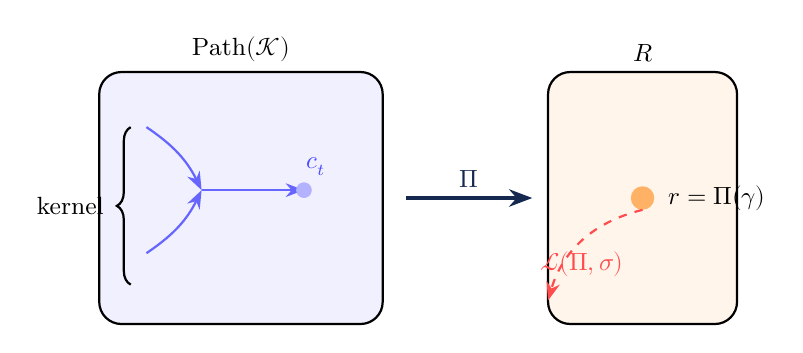
\begin{tikzpicture}[>=Stealth, thick]
  % Path space
  \draw[rounded corners=8pt, fill=blue!6]
    (-3.8,-1.6) rectangle (-0.2,1.6);
  \node[above] at (-2,1.6) {\small$\mathrm{Path}(\mathcal{K})$};

  % Arrows: paths
  \draw[->, blue!60] (-3.2, 0.9) to[bend left=15] (-2.5, 0.1);
  \draw[->, blue!60] (-3.2,-0.7) to[bend right=15] (-2.5, 0.1);
  \draw[->, blue!60] (-2.5, 0.1) -- (-1.2, 0.1);

  \node[circle, fill=blue!30, inner sep=2pt] at (-1.2,0.1) {};
  \node[right, blue!70] at (-1.3,0.4) {\small$c_t$};

  % Projection arrow
  \draw[->, very thick, deepblue] (0.1,0) -- (1.7,0)
    node[midway, above] {\small$\Proj$};

  % Representation space
  \draw[rounded corners=8pt, fill=orange!8]
    (1.9,-1.6) rectangle (4.3,1.6);
  \node[above] at (3.1,1.6) {\small$R$};
  \node[circle, fill=orange!60, inner sep=3pt] at (3.1,0) {};
  \node[right] at (3.3,0) {\small$r = \Proj(\gamma)$};

  % Kernel bracket
  \draw[decorate, decoration={brace, amplitude=5pt}]
    (-3.4,-1.1) -- (-3.4, 0.9)
    node[midway, left=6pt] {\small kernel};

  % Loss arrow
  \draw[->, dashed, red!70] (3.1,-0.15) to[bend right=30]
    node[below] {\small$\mathcal{L}(\Proj,\sigma)$} (1.9,-1.3);
\end{tikzpicture}
\caption{Projection from path space to representation space.
  Multiple distinct trajectories (the kernel) collapse to a single point $r \in R$.
  The projection loss $\mathcal{L}(\Proj, \sigma)$ measures the semantic
  information discarded by this collapse.}
\label{fig:projection}
\end{figure}

% ------------------------------------------------------------
\subsection{The Invariants as a System}
% ------------------------------------------------------------

The four invariants do not function independently.
They form a mutually reinforcing system in which each implies or
strengthens the others.

Constraint primacy (Axiom~\ref{ax:constraint}) establishes that
systems are defined by their admissible paths, not by their states.
Irreversibility (Axiom~\ref{ax:irrev}) establishes that the admissible
paths accumulate into histories that cannot be reversed without
loss of information.
Trajectory-dependence (Axiom~\ref{ax:traj}) establishes that semantic
content is a property of those histories, not of the terminal states
they reach.
And projection loss (Axiom~\ref{ax:proj}) establishes that any
simplification of the path-structured description into a state-structured
one discards semantic information in a predictable, structured way.

Together, they generate the following general picture.
A system is a space of possibilities, organized by exclusions.
What the system can do is defined by what it cannot do.
As the system evolves, it traces a path through this space —
a path that is irreversible, that constitutes the system's identity,
and that carries semantic content not recoverable from any snapshot
of the system's current position.
Any representation that purports to describe the system
by compressing this path into a state, a vector, a score,
or any other lower-dimensional encoding, does so at the cost of
semantic information — information that is lost systematically
and that generates predictable downstream failures.

% ------------------------------------------------------------
\subsection{Irreducibility of Trajectory Structure}
% ------------------------------------------------------------

The informal claim that history cannot be recovered from current
state is made precise by the following theorem, which shows that
any finite-dimensional encoding of a trajectory system is necessarily
non-injective.

\begin{definition}[Trajectory System]
Let $\mathcal{E}$ be a set of events.
A \emph{trajectory} is a finite sequence
$H_n = (e_0, e_1, \dots, e_n)$ with $e_i \in \mathcal{E}$.
A \emph{trajectory system} is a pair $(\mathcal{H}, \mathcal{F})$
where $\mathcal{H} = \bigcup_{n \geq 0} \mathcal{E}^{n+1}$ and
$S_n = \mathcal{F}(H_n)$ is a state defined as a deterministic
fold over history.
\end{definition}

\begin{definition}[History Distinguishability]
A trajectory system $(\mathcal{H}, \mathcal{F})$ is
\emph{history-distinguishing} if for any two distinct histories
$H \neq H'$, there exists an extension $K$ such that
\[
  \mathcal{F}(H \cdot K) \neq \mathcal{F}(H' \cdot K),
\]
where $\cdot$ denotes concatenation.
\end{definition}

\begin{definition}[Finite Representation]
A \emph{finite representation} of a trajectory system is a map
\[
  \pi : \mathcal{H} \to \mathbb{R}^d
\]
for some finite $d$, such that system evolution can be expressed as
$\pi(H \cdot e) = G(\pi(H), e)$ for a fixed function $G$.
\end{definition}

\begin{theorem}[Irreducibility of Trajectory Structure]
\label{thm:irreducibility}
Let $(\mathcal{H}, \mathcal{F})$ be a history-distinguishing
trajectory system with $|\mathcal{E}| \geq 2$.
Then no finite-dimensional representation
$\pi: \mathcal{H} \to \mathbb{R}^d$ can be injective on $\mathcal{H}$.
Equivalently, any finite representation necessarily identifies
distinct histories:
\[
  \exists\, H \neq H' \quad \text{such that} \quad \pi(H) = \pi(H').
\]
\end{theorem}

\begin{proof}
Assume for contradiction that $\pi$ is injective.
Since $|\mathcal{E}| \geq 2$, the number of distinct histories of
length $n$ satisfies $|\mathcal{E}^n| \geq 2^n$, so $\mathcal{H}$
is countably infinite with unbounded combinatorial complexity.
The update rule $\pi(H \cdot e) = G(\pi(H), e)$ implies that
the system is a finite-state dynamical system up to continuous
encoding in $\mathbb{R}^d$.
By the pigeonhole principle applied to finite-precision
distinguishability in $\mathbb{R}^d$, there exist distinct
histories $H \neq H'$ with $\pi(H) = \pi(H')$.
Extending both by a sequence $K$: since evolution depends only
on $\pi(H)$ and $K$, we have $\pi(H \cdot K) = \pi(H' \cdot K)$.
But the system is history-distinguishing, so there exists $K$
with $\mathcal{F}(H \cdot K) \neq \mathcal{F}(H' \cdot K)$,
contradicting injectivity.
Therefore $\pi$ cannot be injective.
\end{proof}

\begin{corollary}[Projection Loss — Formal Version]
\label{cor:projloss-formal}
Any finite-dimensional encoding of a history-distinguishing
trajectory system necessarily loses information about history
and cannot preserve trajectory identity.
\end{corollary}

\begin{remark}
Theorem~\ref{thm:irreducibility} applies equally to physical
systems governed by irreversible entropy flow (where histories are
continuous field trajectories) and to computational systems defined
by event logs (where histories are discrete event sequences).
In both cases, the finite representation necessarily conflates
distinct trajectories and thereby destroys semantic content
that is carried only at the level of the full history.
This is the formal counterpart of the informal claim that
``no summary captures everything.''
\end{remark}

% ------------------------------------------------------------
\subsection{Compression Bounds for Trajectory Systems}
% ------------------------------------------------------------

Theorem~\ref{thm:irreducibility} establishes that projection loss
is nonzero; the following results quantify how large it must be.

\begin{definition}[Trajectory Entropy]
Let $\mathcal{E}$ be a finite event set with $|\mathcal{E}| \geq 2$.
The number of distinct histories of length $n$ is $|\mathcal{E}|^n$.
The \emph{trajectory entropy at depth $n$} is
\[
  H_n = \log |\mathcal{E}|^n = n \log |\mathcal{E}|.
\]
\end{definition}

\begin{definition}[Compression Map]
A \emph{compression map} is a function
$\pi: \mathcal{H}_n \to \mathcal{Z}$
where $\mathcal{H}_n = \mathcal{E}^n$ and $|\mathcal{Z}| < |\mathcal{H}_n|$.
\end{definition}

\begin{theorem}[Minimum Information Loss]
\label{thm:minloss}
Let $\pi: \mathcal{H}_n \to \mathcal{Z}$ be any compression map.
Then the average information loss satisfies
\[
  \mathbb{E}[\mathrm{loss}] \geq H_n - \log |\mathcal{Z}|.
\]
\end{theorem}

\begin{proof}
Each element $z \in \mathcal{Z}$ corresponds to the preimage set
$\pi^{-1}(z) \subseteq \mathcal{H}_n$.
Since $|\mathcal{Z}| < |\mathcal{H}_n|$, by the pigeonhole principle
at least one class has cardinality greater than one;
the average class size is $|\mathcal{H}_n| / |\mathcal{Z}|$.
The expected uncertainty after compression is at least
\[
  \log \frac{|\mathcal{H}_n|}{|\mathcal{Z}|}
  = H_n - \log |\mathcal{Z}|,
\]
and this quantity represents irrecoverable loss of trajectory
information: it cannot be recovered from $\pi(H)$ by any decoder.
\end{proof}

\begin{corollary}[Linear Growth of Loss]
\label{cor:linearloss}
For any fixed representation size $|\mathcal{Z}|$,
the minimum information loss grows linearly in $n$:
\[
  \mathbb{E}[\mathrm{loss}] = \Omega(n).
\]
\end{corollary}

\begin{remark}
Corollary~\ref{cor:linearloss} has a sharp consequence for
machine learning systems, institutional metrics, and any
fixed-size encoding of a temporal process.
No fixed-size representation can track trajectory structure over
unbounded time without accumulating unbounded error.
The practical manifestations of this bound are distributional shift,
loss of causal coherence, and the failure of summary statistics
to predict long-run behavior.
These failure modes are not implementation defects;
they are consequences of Theorem~\ref{thm:minloss}.
\end{remark}

\newpage

% ============================================================
\section{The Generative View}
% ============================================================

\epigraph{\itshape
  The world is not a collection of objects but a history of exclusions.}{}

The four invariants of Section~2 are not merely analytical tools
for criticizing inadequate models.
They are generative: they determine how systems arise, how they interact,
how they compute, and how they learn.
This section develops the positive account implied by the invariants —
the view of system genesis and system behavior that follows from taking
constraint primacy, irreversibility, trajectory-dependence, and
projection loss as foundational.

% ------------------------------------------------------------
\subsection{Systems as Constrained Possibility Spaces}
% ------------------------------------------------------------

Under constraint primacy, a system is not a collection of objects or
an ensemble of states.
It is a structured space of possibilities: a set of configurations
equipped with a constraint structure that determines which transitions
between configurations are admissible.
The system's ``content'' — what it contains, what it can express,
what it can compute — is the set of admissible paths through this space.

This has a geometric interpretation that is both precise and fertile.
The constraint structure $(\Cfg, \Trans, \mathcal{F})$ defines a
directed graph on $\Cfg$, and the admissible paths are the directed
walks through this graph.
The ``shape'' of the system — its topology, its degeneracy structure,
its capacity for self-reference — is the shape of this directed graph.

Different types of constraint structures generate systems with
qualitatively different behaviors.
A constraint structure in which every configuration has many successors
is a system with high branching factor — high expressive capacity but
also high sensitivity to initial conditions, since small differences
in starting configuration lead to divergent long-run trajectories.
A constraint structure in which successor configurations are tightly
controlled — few admissible transitions — is a system with low
branching factor, stable long-run behavior, and strong path-dependence:
what the system can be in the future is sharply constrained
by what it has been in the past.
Natural languages occupy an intermediate regime, as do biological genomes
and — importantly for the analysis of Section~4 — the human conceptual
repertoire as it develops through learning.

The generative power of this picture lies in its ability to describe
the emergence of structure without presupposing it.
Complex configurations — organized structures, coherent semantic units,
stable dynamical attractors — arise not because they are objectives
toward which the system is optimized but because the constraint structure
makes them attractors of the admissible path space:
regions of configuration space into which many paths lead and from which
few paths escape.
They are fixed points not of an objective function but of a
trajectory-generating process.

% ------------------------------------------------------------
\subsection{Interaction as Progressive Elimination}
% ------------------------------------------------------------

If a system is a space of possibilities organized by exclusions,
then interaction between two systems is the mutual imposition of
additional constraints — a progressive narrowing of the joint
possibility space.

\begin{definition}[Interaction]
Let $\mathcal{K}_1 = (\Cfg_1, \Trans_1, \mathcal{F}_1)$ and
$\mathcal{K}_2 = (\Cfg_2, \Trans_2, \mathcal{F}_2)$ be constraint structures.
Their \emph{interaction} is the constraint structure
$\mathcal{K}_1 \otimes \mathcal{K}_2 = (\Cfg_1 \times \Cfg_2, \Trans_{12}, \mathcal{F}_{12})$
where $(c_1, c_2) \to (c'_1, c'_2) \in \Trans_{12}$ iff
$(c_1, c'_1) \in \Trans_1$, $(c_2, c'_2) \in \Trans_2$,
and the pair is consistent with an interaction protocol
$\mathcal{I} \subseteq \Trans_1 \times \Trans_2$.
\end{definition}

The interaction protocol $\mathcal{I}$ is the formal counterpart of
what in physics is called a coupling: it specifies which transitions
in one system can co-occur with which transitions in the other.
Tight coupling ($\mathcal{I}$ small) produces strong mutual constraint
and rapid equilibration — the two systems quickly reduce their
joint possibility space.
Loose coupling ($\mathcal{I}$ large) preserves more independence —
the joint system retains more of the product of the individual
possibility spaces.

This picture of interaction as progressive elimination has consequences
for the theory of communication.
Two systems communicate when their interaction protocol allows the
transitions of one to select among the transitions of the other.
Successful communication is not the transfer of a symbolic object
from one system to another but the coordinated narrowing of
mutual possibility spaces — a process whose success is measured by
the degree to which the receiving system's subsequent trajectories
are constrained in the way the transmitting system intended.
Projection loss applies here: the transmitted message is a projection
of the transmitter's trajectory, and the receiver reconstructs a
trajectory in its own possibility space that may differ systematically
from the transmitter's in ways determined by the structure
of the respective constraint structures and the coupling between them.

% ------------------------------------------------------------
\subsection{Computation as History Construction}
% ------------------------------------------------------------

The generative view makes computation a species of history construction.
A computation is an admissible path through the constraint structure
of a computing device, initiated at a specified starting configuration
(encoding the program and input) and terminating at a configuration
from which the output is read.
The computation's result is not its terminal configuration alone
but the entire path — because, by Theorem~\ref{thm:semantic},
the semantic content of the computation (what it means, what it proves,
what it implements) is a property of the trajectory,
not of the terminal state.

This perspective generates a novel account of computational equivalence.
Two computations are equivalent not when they produce the same output
but when their trajectories are related by a structure-preserving map
that respects the semantic function.
A compilation, for example, is such a map: a compiler translates a
path through the constraint structure of a high-level language into
a path through the constraint structure of machine code,
preserving (under correct compilation) the semantic function
while changing the constraint structure in which the path is traced.

The irreversibility axiom implies that computation is not logically
reversible in general.
This is not a consequence of physical resource constraints —
it is a structural feature of computation viewed as history
construction.
The path $\gamma_t$ that produced the current state $c_t$
is not recoverable from $c_t$ alone, precisely because the map
$\gamma_t \mapsto c_t$ is many-to-one.
This has implications for the design of programming languages,
for the theory of program verification, and for the analysis of
cryptographic protocols, all of which will be developed in
the domain analysis of Section~4.

% ------------------------------------------------------------
\subsection{Learning as Trajectory Shaping}
% ------------------------------------------------------------

Learning, under the generative view, is the process by which a system
modifies its constraint structure in response to its history.
This is importantly different from the standard picture of learning
as the adjustment of parameters within a fixed model architecture
to minimize a loss function.

\begin{definition}[Learning as Constraint Modification]
A \emph{learning process} on a system $S$ with constraint structure
$\mathcal{K}$ is a sequence of constraint structures
$\mathcal{K}_0, \mathcal{K}_1, \mathcal{K}_2, \ldots$
where $\mathcal{K}_0 = \mathcal{K}$ and each $\mathcal{K}_{t+1}$
is a modification of $\mathcal{K}_t$ determined by the history
$\gamma_t \in \mathrm{Path}(\mathcal{K}_t)$ accumulated up to time $t$.
\end{definition}

On this account, learning does not optimize a fixed objective within
a fixed possibility space.
It reshapes the possibility space itself.
The space of what the system can subsequently do is altered by
the history of what it has done — not merely by summary statistics
of that history, but by the history's structure.
This means that learning histories matter: two systems that have
seen the same data in different orders, under different constraint
structures, will in general have different subsequent possibility spaces,
even if their current output distributions are identical.

The failure modes of standard machine learning —
distributional shift, adversarial vulnerability, catastrophic forgetting —
all have natural explanations in this framework.
Distributional shift is the mismatch between the constraint structure
under which learning occurred and the constraint structure of the
deployment environment.
Adversarial vulnerability is the exploitation of paths that are
admissible under the learned constraint structure but were not
sampled during training.
Catastrophic forgetting is the erasure of accumulated history
by a learning update that treats the current state as the only
relevant information.
Each failure mode corresponds to a specific violation of one of
the four invariants.

\newpage

% ============================================================
\section{Domains as Projections}
% ============================================================

\epigraph{\itshape
  The same river cannot be stepped in twice, but neither can it
  be correctly described by any single crossing.}{}

The four invariants of Section~2 and the generative principles
of Section~3 manifest across distinct domains — language, computation,
cognition, and physics — not as analogies or metaphors but as
structural projections.
Each domain instantiates the same underlying constraint-trajectory-
irreversibility architecture through a different representational lens.
Each domain's specific technical vocabulary and formal tools are
adaptations of that underlying structure to the particular nature of
its objects of study.
And each domain's characteristic failure modes, as Section~5 will show,
are instances of the same class of projection-loss errors.

This section is organized as a sequence of domain analyses,
each identifying the constraint structure, the admissible paths,
the semantic function, and the specific form of projection loss
characteristic of the domain.
The reader should note that the subsections are not independent:
the language analysis motivates the formal vocabulary used in the
computation analysis, which in turn motivates the cognitive analysis,
and the physical analysis provides the broadest context within
which all three are embedded.

% ------------------------------------------------------------
\subsection{Language and Symbol Systems}
% ------------------------------------------------------------

Language is the clearest and most familiar instantiation of the
constraint-primacy view.
A natural language is not a collection of meaningful units —
words, sentences, texts — but a constraint structure on sequences of
symbols, where the constraints are phonological, morphological,
syntactic, and pragmatic, and where the admissible paths through
this constraint structure are the grammatical and contextually
appropriate utterances.

The constraint structure of language is multi-layered in a precise sense.
Each layer imposes constraints on a different aspect of the symbol
sequence, and the layers interact: phonological constraints restrict
which morphemes can adjoin, morphological constraints restrict which
words can be formed, syntactic constraints restrict which phrases and
clauses can be combined, and pragmatic constraints restrict which
combinations are felicitous in a given communicative context.
The constraint structures at each level are not independent;
they form a hierarchy in which each level's admissible transitions
are defined partly in terms of the admissible paths at lower levels.

\begin{definition}[Linguistic Constraint Hierarchy]
A \emph{linguistic constraint hierarchy} is a sequence
$\mathcal{K}_1, \mathcal{K}_2, \ldots, \mathcal{K}_n$ of constraint
structures where the configuration space of each $\mathcal{K}_{i+1}$
is a subset of $\mathrm{Path}(\mathcal{K}_i)$:
each level's configurations are paths at the level below.
\end{definition}

Under this definition, a word is an admissible path through the
phonological constraint structure; a phrase is an admissible path
through the morphosyntactic constraint structure whose configurations
are words; a sentence is an admissible path through the syntactic
constraint structure whose configurations are phrases; and so on.
Meaning — semantic content — is a function on paths through the highest
level of the hierarchy, not on configurations at any single level.
This is why the meaning of a sentence is not recoverable from
the set of words it contains, regardless of how those words are
defined in isolation: the trajectory of their combination,
constrained at every level of the hierarchy, is constitutive of meaning.

Writing systems — orthographies — are projections in the formal sense
of Definition 2.12.
An orthography projects the phonological constraint structure
(the space of admissible sound sequences) onto a graphemic constraint
structure (the space of admissible letter and character sequences).
This projection is never fully faithful: all orthographies incur
projection loss, discarding some phonological distinctions
(stress, intonation, allophonic variation) while possibly introducing
distinctions absent in the phonological structure (etymological spellings,
heteronyms, homographs).
The specific pattern of projection loss is characteristic of the
orthographic system and generates predictable difficulties for learners.

Constructed and cryptographic writing systems — symbol sets designed
for purposes other than faithful phonological transcription —
are most perspicuously understood as deliberate manipulation of
the projection map between levels of the linguistic constraint hierarchy.
A writing system that assigns symbols to semantic primitives rather than
phonemes projects the phonological level entirely, retaining the
semantic level directly.
Such a projection minimizes projection loss at the semantic level
while maximizing it at the phonological level — a trade-off whose
consequences are systematic: the symbol set is semantically transparent
but phonologically opaque, and learning it requires direct access
to the semantic constraint structure rather than phonological decoding.

The process of translation between natural languages is, under this
framework, a projection between two distinct linguistic constraint
hierarchies.
The translation map $T: \mathrm{Path}(\mathcal{K}_L) \to \mathrm{Path}(\mathcal{K}_{L'})$
incurs projection loss whenever the two hierarchies differ in the
distinctions they grammaticalize.
Languages that grammaticalize aspect (the internal structure of events)
lose aspectual information when translated into languages without
grammaticalized aspect; languages with grammaticalized evidentiality
lose information about the epistemic source of claims when translated
into languages without it.
These losses are structural — they follow from the geometry of the
projection — and no degree of translator skill can recover
what the constraint structure of the target language does not
have the resources to encode.

This has a consequence for the theory of language learning and
immersion that is often observed empirically but rarely given
a formal account.
When a learner acquires a second language through sustained immersion —
through reading, interaction, and productive use — rather than through
translation from the first language, the learner is constructing
a distinct linguistic constraint structure rather than building a
translation map from the existing one.
The resulting constraint structure is genuinely different in its
organization of the possibility space, not merely a relabeling of
the first language's structure in new vocabulary.
The learner who has achieved this construction can navigate
the second language's constraint structure directly,
without incurring the systematic projection losses of translation.

This is also why the epistemological value of deliberate language
immersion extends beyond linguistic competence to affect
the learner's constraint structure for thought itself —
a point to which the analysis of cognitive frameworks in §4.3 returns.

% ------------------------------------------------------------
\subsection{Computation and Interaction Design}
% ------------------------------------------------------------

The computational domain is the one in which the constraint-trajectory
framework has its most direct formal instantiation.
A computation, as noted in §3.3, is an admissible path through the
constraint structure of a computing device.
The device's constraint structure — its instruction set, its memory
model, its I/O specification — determines the space of admissible
computations; any program is a description of a path through this space.

The most consequential formal property of computation under this
framework is \emph{computational irreducibility}: for many computations,
there exists no representation of their trajectory shorter than the
trajectory itself.
The only way to determine the outcome is to execute the path.
This is the computational counterpart of Theorem~\ref{thm:identity}:
the identity of a computation — what it computes, what side effects it
produces, what resources it consumes — is a function of its full trajectory,
not of any compressed representation of it.

\begin{definition}[Computationally Irreducible Path]
An admissible path $\gamma$ in a constraint structure $\mathcal{K}$
is \emph{computationally irreducible} with respect to a semantic function
$\sigma$ if there is no path $\gamma'$ with $|\gamma'| < |\gamma|$
and $\sigma(\gamma') = \sigma(\gamma)$: no shorter path produces
the same semantic result.
\end{definition}

Computational irreducibility has immediate implications for the design
of interactive systems.
A game — understood as a constraint structure on player action sequences —
is interesting to the extent that it is computationally irreducible:
the player cannot shortcut the trajectory of play, cannot compute
the ``correct move'' without exploring the path space.
A game whose optimal strategy can be computed ahead of time —
whose trajectory is reducible to a state — is, in the precise sense
of this framework, not a game but a puzzle: a constraint structure
in which the admissible paths collapse to a single semantically
interesting trajectory.

This distinction — between games as genuinely irreducible path spaces
and puzzles as reducible ones — applies beyond recreational systems.
Software user interfaces, programming languages, and interactive
computational environments are all constraint structures on user
action sequences.
Their design quality, from the perspective of this framework,
is measured by the relationship between their admissible path space
and the space of user intentions.
A well-designed interface is one whose constraint structure is
aligned with the user's constraint structure for action —
where the paths the user intends to take are admissible and efficient,
and where the paths the user does not intend are inadmissible or costly.
Poor interface design is, on this account, a projection mismatch:
the constraint structure of the interface and the constraint structure
of the user's intentions have incompatible projections onto the space
of available interactions.

Event-sourced architectures in software engineering are the most direct
practical instantiation of the trajectory-primacy view.
In an event-sourced system, the primary data structure is not the current
state of the system but the ordered log of events that produced it:
the history $\gamma_t$.
The current state is derived from this log by applying a projection.
This architectural choice directly implements Axiom~\ref{ax:irrev}:
identity is the history, not the current configuration.
Event-sourced systems are correspondingly more robust to the failure
modes described in Section~5 — in particular to identity fragility
and to the loss of causal structure — because they retain the
trajectory rather than compressing it.

Deterministic replay — the capacity to reconstruct any past state of
a system by replaying its event log from the beginning — is, under
this framework, the implementation of the map $\gamma_t \mapsto c_t$
for arbitrary $t$.
It is precisely what makes history available as a resource for
debugging, auditing, and understanding system behavior.
Systems that discard their event logs in favor of snapshot-based
state storage have traded the ability to reconstruct identity
for storage efficiency — an instance of the projection-efficiency
trade-off that is the practical form of the projection-loss problem.

The Spherepop event calculus — an irreversible computation model
developed within the RSVP framework — is a formal system designed
to make trajectory-primacy constitutive rather than optional.
In Spherepop, events are first-class objects; states are derived;
and the semantic function of a computation is explicitly defined
on event sequences rather than terminal configurations.
Irreversibility is enforced structurally: the calculus has no inverse
for event application, so the history cannot be erased or
reconstructed from the current state alone.
This makes the calculus a direct formal implementation of
Axioms~\ref{ax:irrev} and \ref{ax:traj},
and makes its computational properties — in particular,
the properties of fixed-point computation and self-reference —
direct consequences of the general theory developed in Section~2.

% ------------------------------------------------------------
\subsection{Cognitive and Artificial Intelligence Frameworks}
% ------------------------------------------------------------

The analysis of intelligence — both biological and artificial —
under the constraint-trajectory framework produces a reorientation
of foundational questions.
The standard question in cognitive science and AI research is:
what objective function does the intelligent system optimize?
The reoriented question is: what constraint structure does the
intelligent system inhabit, and how does it navigate the admissible
paths of that structure given its history?

These are not merely different formulations of the same question.
They generate different research programs and different predictions
about the conditions under which intelligent behavior succeeds or fails.

The objective-function picture predicts that an intelligent system
improves monotonically with the quality of the objective function
and the fidelity of the optimization.
The constraint-trajectory picture predicts that the system's behavior
is determined by the interaction between its current constraint structure
and its accumulated history, and that improvement requires not better
optimization but appropriate modification of the constraint structure
— learning in the sense of Definition~3.4 rather than parameter tuning.

\begin{proposition}[Sparse Heuristics as Emergent Constraint]
\label{prop:heuristics}
In a constraint structure $\mathcal{K}$ with large admissible path space,
a learning process that successfully shapes trajectories will converge
toward a set of heuristics that are not explicit objectives but
implicit constraints: they eliminate large regions of the admissible
path space without being derived from an objective function.
\end{proposition}

The informal content of Proposition~\ref{prop:heuristics} is that
expertise is the internalization of constraint.
An expert in any domain — a chess player, a physician, a programmer —
does not search the full admissible path space with an explicit
objective function.
The expert has, through the accumulation of trajectory history,
modified their constraint structure to make large regions of the
admissible path space effectively inadmissible.
Expert intuition is not a shortcut to objective-function optimization;
it is a reconfigured constraint structure.

This has direct consequences for the theory of artificial intelligence.
Current large language models and related systems are trained to
approximate a statistical objective — next-token prediction or
preference alignment — over a fixed constraint structure
(the structure of natural language sequences).
They are, in the terminology of this framework, trajectory-sampling
devices rather than constraint-modifying devices:
they sample admissible paths through a learned approximation to
the statistical structure of language, but they do not modify
the constraint structure itself in response to the history of their
outputs.

This is the source of their characteristic failure modes:
they hallucinate (sample paths admissible under the statistical
constraint structure but not under the factual one),
they are inconsistent across contexts (the constraint structure
they approximate is a projection of the full context that varies
with the projection map of the prompt),
and they fail catastrophically on out-of-distribution inputs
(the learned constraint structure does not extend to regions of
the path space not sampled during training).

Geometric approaches to cognition — understanding conceptual
structure as a geometry on a space of mental configurations —
are compatible with the constraint-trajectory framework when
they are interpreted correctly.
The mental configuration space is a constraint structure;
the geometry is the metric on that space induced by the
pattern of admissible transitions.
Conceptual change — learning, inference, discovery — is modification
of the constraint structure, which may change the geometry
of the configuration space as well as its content.

The alignment problem in artificial intelligence — how to ensure that
an AI system behaves in accordance with human values and intentions —
is, under this framework, a constraint-matching problem:
how to ensure that the AI system's constraint structure is appropriately
coupled to the constraint structure of human normative practice.
This is a different problem from objective-function alignment,
and it calls for different solutions.
Objective-function alignment attempts to specify, in advance and in
scalar form, what the system should optimize.
Constraint-structure alignment attempts to ensure that the system's
admissible path space is appropriately related to the admissible
path space of human action and judgment.

The latter is more robust for the reasons identified in Section~2:
it does not presuppose a complete and correct specification of
the objective, does not generate Goodhart effects when the
specification is imperfect, and preserves the semantic content
of the system's behavior rather than compressing it into a scalar value.

% ------------------------------------------------------------
\subsection{Physical and Cosmological Models}
% ------------------------------------------------------------

The physical domain is in one sense the most remote from everyday
applications of the constraint-trajectory framework,
and in another sense the most fundamental.
It is the most remote because the relevant constraint structures
— the laws of physics — are fixed by nature and not subject to design
or modification in the way that linguistic, computational, or
cognitive constraint structures are.
It is the most fundamental because all other constraint structures
are ultimately embedded in the physical one: the constraint structures
of language, computation, and cognition are implemented in physical
systems and must be consistent with the physical constraint structure.

The physical constraint structure is irreversible in the most
fundamental sense: the second law of thermodynamics asserts that
the entropy of an isolated system is non-decreasing in time.
Entropy, under the statistical mechanical interpretation,
is a measure of projection loss: it measures how much information
about the microscopic trajectory is discarded when the trajectory
is projected onto macroscopic observables.

\begin{theorem}[Entropy as Projection Loss]
\label{thm:entropy}
In the statistical mechanical setting, the thermodynamic entropy
$S(t) = -k_B \sum_i p_i \log p_i$
is the projection loss incurred by projecting the microscopic
trajectory onto the macroscopic state description,
where $p_i$ is the probability of microscopic configuration $i$
consistent with the macroscopic state at time $t$.
\end{theorem}

The proof of Theorem~\ref{thm:entropy} is standard and follows
from the identification of entropy with the logarithm of the
number of microscopic configurations consistent with the macroscopic
state — which is precisely the logarithm of the size of the
kernel of the projection map from microscopic configurations
to macroscopic states.

The second law of thermodynamics is therefore a special case of
Theorem~\ref{thm:projloss} applied to the physical constraint structure:
projection loss is non-decreasing in time because the projection map
from microscopic trajectories to macroscopic states is many-to-one
and because physical evolution moves the system through the
high-entropy (large-kernel) regions of configuration space.

The RSVP (Relativistic Scalar-Vector Plenum) field-theoretic
framework extends this analysis to cosmological scales.
In RSVP, spacetime geometry is not a fixed background on which
matter evolves but is itself an evolving constraint structure:
the geometry of space and time at any moment is the result of
the accumulated trajectory of the plenum field up to that moment.
Space and time are emergent from constraint relaxation —
from the progressive narrowing of the possibility space of
field configurations — rather than being primitive.

This is the physical analogue of the claim that identity is path-dependent:
the structure of spacetime at time $t$ is not given independently
of the trajectory of the plenum field that produced it.
The cosmological implications are significant.
The large-scale structure of the universe — the distribution of
galaxies, the homogeneity of the cosmic microwave background,
the apparent flatness of spatial slices — are not arbitrary
initial conditions but consequences of the constraint structure
of the plenum and the trajectory it has traced.
Explaining these structures requires an account of the trajectory,
not merely of the current state.

The relationship between physical and informational systems —
between the physical constraint structure and the constraint structures
of computation and cognition — is not metaphorical.
Both are constraint structures in the formal sense of Definition~2.1,
and both are subject to the same invariants.
The projection from physical to informational constraint structure
incurs projection loss in the same formal sense as the projection
from linguistic to graphemic constraint structure.
The difference is one of scale and of the mechanisms by which
the constraint structures are implemented and modified.

\begin{figure}[h]
\centering
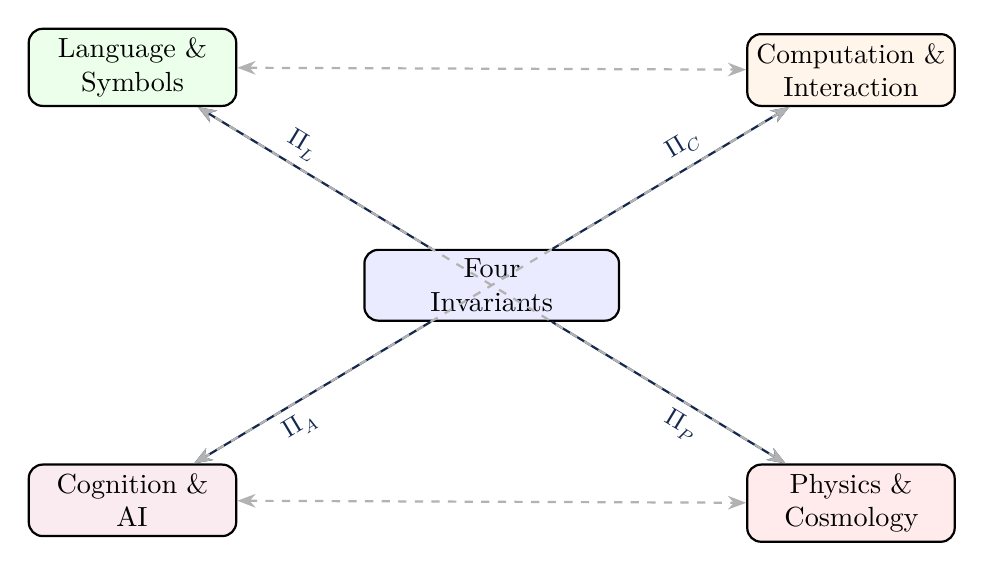
\begin{tikzpicture}[>=Stealth, thick, node distance=2.2cm]
  % Central node
  \node[draw, rounded corners=5pt, fill=blue!8,
        text width=3cm, align=center] (inv)
    {Four\\Invariants};

  % Domain nodes
  \node[draw, rounded corners=5pt, fill=green!8,
        text width=2.4cm, align=center, above left=1.8cm and 1.6cm of inv] (lang)
    {Language \&\\Symbols};
  \node[draw, rounded corners=5pt, fill=orange!8,
        text width=2.4cm, align=center, above right=1.8cm and 1.6cm of inv] (comp)
    {Computation \&\\Interaction};
  \node[draw, rounded corners=5pt, fill=purple!8,
        text width=2.4cm, align=center, below left=1.8cm and 1.6cm of inv] (cog)
    {Cognition \&\\AI};
  \node[draw, rounded corners=5pt, fill=red!8,
        text width=2.4cm, align=center, below right=1.8cm and 1.6cm of inv] (phys)
    {Physics \&\\Cosmology};

  % Projection arrows
  \draw[->, deepblue] (inv) -- node[above left, sloped, font=\small]
    {$\Proj_L$} (lang);
  \draw[->, deepblue] (inv) -- node[above right, sloped, font=\small]
    {$\Proj_C$} (comp);
  \draw[->, deepblue] (inv) -- node[below left, sloped, font=\small]
    {$\Proj_A$} (cog);
  \draw[->, deepblue] (inv) -- node[below right, sloped, font=\small]
    {$\Proj_P$} (phys);

  % Interaction arrows between domains
  \draw[<->, gray!60, dashed] (lang) -- (comp);
  \draw[<->, gray!60, dashed] (comp) -- (cog);
  \draw[<->, gray!60, dashed] (cog) -- (phys);
  \draw[<->, gray!60, dashed] (phys) -- (lang);
\end{tikzpicture}
\caption{The four invariants project onto four domain families.
  Each projection map $\Proj_D$ is faithful to the invariants
  while incurring domain-specific projection loss.
  Dashed arrows indicate inter-domain structural homomorphisms.}
\label{fig:domains}
\end{figure}

\newpage

% ============================================================
\section{Category-Theoretic Formulation of Trajectory Systems}
% ============================================================

\epigraph{\itshape
  A functor that forgets is not neutral — it is a commitment to ignorance.}{}

The domain analyses of the preceding section share a common
abstract skeleton: each domain defines a category of histories,
a functor into a state space, and a projection functor into
a finite representation.
This section makes that skeleton explicit, establishing the
categorical counterparts of the metric results of
Theorems~\ref{thm:irreducibility} and~\ref{thm:minloss}.

% ------------------------------------------------------------
\subsection{The Category of Histories}
% ------------------------------------------------------------

\begin{definition}[Category of Histories]
Let $\mathbf{Hist}$ be the category where:
\begin{itemize}
  \item Objects are finite event histories $H_n \in \mathcal{E}^n$
    for $n \geq 0$.
  \item Morphisms $f: H_n \to H_{n+1}$ are append operations:
    $f(H_n) = H_n \cdot e_{n+1}$ for some event $e_{n+1} \in \mathcal{E}$.
  \item Composition is concatenation; the identity on $H_n$
    is the empty append.
\end{itemize}
\end{definition}

\begin{proposition}[History as Free Monoid]
The category $\mathbf{Hist}$ is generated by the free monoid
$\mathcal{E}^*$ under concatenation.
Every object is reachable from the empty history $H_0 = ()$
by a finite sequence of morphisms.
\end{proposition}

\begin{definition}[State Functor]
A \emph{state functor} is a mapping
$F: \mathbf{Hist} \to \mathbf{State}$
such that $F(H_n) = S_n$ and $F(f) = \delta$,
where $\delta$ is the deterministic state update rule.
\end{definition}

\begin{definition}[Irreversible Morphism]
A morphism $f: H_n \to H_{n+1}$ in $\mathbf{Hist}$ is
\emph{irreversible} if no inverse morphism
$f^{-1}: H_{n+1} \to H_n$ exists in $\mathbf{Hist}$.
\end{definition}

Since the append operation strictly increases the length of a
history, every morphism in $\mathbf{Hist}$ is irreversible.
This is the categorical expression of Axiom~\ref{ax:irrev}:
the category of histories has no inverses, only extensions.

% ------------------------------------------------------------
\subsection{Projection Functors and Non-Faithfulness}
% ------------------------------------------------------------

\begin{definition}[Projection Functor]
A \emph{projection functor} is a functor
$\pi: \mathbf{Hist} \to \mathbf{Rep}$
into a category $\mathbf{Rep}$ of finite representations.
\end{definition}

\begin{theorem}[Non-Faithfulness of Finite Projections]
\label{thm:nonfaithful}
Any projection functor $\pi: \mathbf{Hist} \to \mathbf{Rep}$
into a category with finitely many distinct morphisms is not faithful.
That is, there exist distinct morphisms $f \neq g$ in $\mathbf{Hist}$
such that $\pi(f) = \pi(g)$.
\end{theorem}

\begin{proof}
$\mathbf{Hist}$ contains infinitely many distinct morphisms
(one for each finite event sequence), since $|\mathcal{E}| \geq 2$.
$\mathbf{Rep}$ contains only finitely many distinct morphisms
by hypothesis.
Any functor from an infinite morphism set to a finite one must
identify distinct morphisms.
Therefore $\pi$ is not faithful.
\end{proof}

\begin{remark}
Theorem~\ref{thm:nonfaithful} is the categorical formulation of
projection loss.
A faithful functor preserves all distinctions; a non-faithful functor
collapses them.
Every finite representation of the trajectory system is a
non-faithful projection, and the collapsed distinctions are
precisely the lost semantic content.
This provides a categorical foundation for Corollary~\ref{cor:projloss-formal}:
projection loss is not merely a quantitative limitation
but a categorical one.
\end{remark}

% ------------------------------------------------------------
\subsection{The Refuse Operator as a Categorical Boundary}
% ------------------------------------------------------------

The Refuse operator — the mechanism by which inadmissible events
are rejected from the history — has a natural categorical formulation.

\begin{definition}[Admissibility Functor]
An \emph{admissibility functor} is a functor
$\mathcal{A}: \mathbf{Hist} \to \mathbf{2}$
where $\mathbf{2} = \{0 \to 1\}$ is the arrow category,
with $\mathcal{A}(H_n) = 1$ if $H_n$ is admissible and
$\mathcal{A}(H_n) = 0$ otherwise.
\end{definition}

The Refuse operator acts on proposed morphisms
$f: H_n \to H_{n+1}$ by checking whether $H_{n+1}$ is
admissible given $H_n$.
If $\mathcal{A}(H_{n+1}) = 0$, the morphism is replaced by
the identity $\mathrm{id}_{H_n}$: the history is not extended.
This is the categorical counterpart of the infinite-action
boundary condition in the variational formalism of
Section~\ref{sec:lagrangian}.

\begin{proposition}[Categorical Refuse]
\label{prop:catrefuse}
Let $\mathcal{A}$ be an admissibility functor.
The Refuse operator $\mathcal{R}$ is the natural transformation
$\mathcal{R}: \mathrm{Id}_{\mathbf{Hist}} \Rightarrow \mathcal{A}^{-1}(1)$
that maps inadmissible morphisms to identity morphisms and
admissible morphisms to themselves.
The image of $\mathcal{R}$ is a subcategory of $\mathbf{Hist}$
containing only admissible histories.
\end{proposition}

\begin{proof}
For any morphism $f: H_n \to H_{n+1}$:
if $\mathcal{A}(H_{n+1}) = 1$, $\mathcal{R}(f) = f$;
if $\mathcal{A}(H_{n+1}) = 0$, $\mathcal{R}(f) = \mathrm{id}_{H_n}$.
The result is a well-defined endofunctor on the subcategory
of admissible objects, since admissible morphisms compose to
admissible morphisms by the closure property of $\mathcal{A}$.
\end{proof}

\newpage

% ============================================================
\section{Physical--Computational Correspondence}
\label{sec:phys-comp}
% ============================================================

\epigraph{\itshape
  Two systems may speak the same structural language
  without sharing a single physical component.}{}

Both the RSVP framework and the Spherepop architecture
instantiate trajectory systems under different representational
constraints.
This section makes the correspondence explicit through a shared
categorical structure, without overclaiming identity.

% ------------------------------------------------------------
\subsection{Two Instantiations of the Same Structure}
% ------------------------------------------------------------

In the RSVP framework, histories correspond to continuous evolution
of the entropy density field $\mathcal{S}(x,t)$ and vector field
$\vec{V}(x,t)$ over the spatial domain $\Omega$.
The ``events'' are infinitesimal field increments;
the state at time $t$ is the entire field configuration,
which is a functional of the trajectory
$\{\mathcal{S}(x,s)\}_{s \leq t}$.

In Spherepop, histories correspond to discrete event sequences
$H_n = (e_0, e_1, \dots, e_n)$.
The state $S_n = \mathcal{F}(H_n)$ is a deterministic fold
over the event log.

In both cases:
\begin{enumerate}
  \item evolution is strictly path-dependent,
  \item no global state exists independent of history,
  \item projection of histories into reduced representations
    induces loss — continuous in the RSVP case
    (thermodynamic coarse-graining),
    discrete in the Spherepop case (finite-state encoding).
\end{enumerate}

The following table makes the structural parallelism explicit.

\begin{center}
\begin{tabular}{lccc}
\toprule
\textbf{Feature} & & \textbf{RSVP} & \textbf{Spherepop} \\
\midrule
Fundamental unit      && Entropy-vector field & Event history $H_n$ \\
State definition      && $\mathcal{S}(x,t)$, functional of trajectory & $S_n = \mathcal{F}(H_n)$ \\
Evolution rule        && $\vec{g} \approx -\nabla \mathcal{S}$ & $\delta(S_{n-1}, e_n) \to S_n$ \\
Irreversibility       && $d\mathcal{S}/dt \geq 0$ & Append-only history \\
Refusal boundary      && Entropic flux limit & Refuse operator $\mathcal{R}$ \\
Structural framework  && Global field sections & Local event manifold \\
\bottomrule
\end{tabular}
\end{center}

\begin{proposition}[Structural Correspondence]
\label{prop:correspondence}
RSVP and Spherepop define functors from trajectory categories
into distinct state spaces — continuous and discrete respectively —
that preserve irreversibility but differ in representation.
They are therefore \emph{structurally analogous} as instances of
the same categorical framework but are not strictly isomorphic,
since their objects, morphisms, and composition laws are
drawn from different mathematical structures
(function spaces vs.\ discrete monoids).
\end{proposition}

The significance of Proposition~\ref{prop:correspondence}
is that the RSVP–Spherepop relationship is not a metaphor
and not an identity.
It is a structural homomorphism: both systems are instances of
the trajectory-category framework, projecting into different
representation spaces through functors that share the property
of irreversibility-preservation.
The failure modes of each system under projection are therefore
the same failure modes, instantiated through different mechanisms.

% ------------------------------------------------------------
\subsection{Gravity as Entropic Gradient}
% ------------------------------------------------------------

In the RSVP model, gravitational acceleration emerges as a gradient
of the entropy density field:
\[
  \vec{g}(x,t) \approx -\nabla \mathcal{S}(x,t).
\]
This is not a conventional derivation of gravity but an
emergentist account: what is standardly modeled as a force
is, in the RSVP framework, the directional bias imposed on
local field evolution by the global entropy gradient.
The field cannot evolve ``uphill'' in entropy without external
energy input; the resulting directionality is what
macroscopic observers register as gravitational attraction.

The computational parallel is direct.
In Spherepop, the state transition $\delta(S_{n-1}, e_n) \to S_n$
is directional in exactly the same sense:
it maps the current state to the next by applying an event,
and this map is not invertible.
The ``direction'' of computation — the fact that programs
run forward and cannot be reversed without explicit mechanism
— is the computational counterpart of entropic directionality
in the RSVP plenum.

Both structures instantiate the same underlying principle:
Axiom~\ref{ax:irrev}, irreversibility, is not a feature
of one domain borrowed by analogy into another.
It is a property of the constraint structure itself,
which manifests as entropic flow in the physical domain
and as event accumulation in the computational one.

% ------------------------------------------------------------
\subsection{Discrete Realization and Loss Bounds}
% ------------------------------------------------------------

The correspondence established in \S\ref{sec:phys-comp} between
RSVP field dynamics and Spherepop event histories can be made
formally precise by exhibiting a discretization map from
continuous trajectories to discrete histories and deriving
the associated loss bounds.
This converts the structural analogy of Proposition~\ref{prop:correspondence}
into a provable functorial reduction.

\begin{definition}[Continuous Trajectory]
Let $\mathcal{F}$ denote the space of admissible field configurations —
entropy density $\mathcal{S}(x,t)$ and vector field $\vec{V}(x,t)$
over $\Omega$.
A \emph{continuous trajectory} is a map
\[
  \Gamma : [0,T] \to \mathcal{F}
\]
satisfying the dynamical constraints of the RSVP field equations.
\end{definition}

\begin{definition}[Discretization Map]
Fix a temporal resolution $\Delta > 0$.
A \emph{discretization map} is a function
\[
  \mathcal{D}_\Delta : \{\Gamma\} \to \mathcal{H}
\]
that assigns to each continuous trajectory $\Gamma$ a discrete history
$\mathcal{D}_\Delta(\Gamma) = (e_0, e_1, \dots, e_n)$,
where each event $e_i$ encodes the field transition over the interval
$[i\Delta, (i+1)\Delta]$ via a symbolic encoding of field variation.
\end{definition}

\begin{proposition}[Non-Faithfulness of Discretization]
\label{prop:nonfaith-disc}
For any finite $\Delta > 0$, the map $\mathcal{D}_\Delta$ is not injective:
\[
  \exists\, \Gamma \neq \Gamma' \quad \text{such that} \quad
  \mathcal{D}_\Delta(\Gamma) = \mathcal{D}_\Delta(\Gamma').
\]
\end{proposition}

\begin{proof}
The space of continuous trajectories over $[0,T]$ is infinite-dimensional,
while the image of $\mathcal{D}_\Delta$ has cardinality at most
$|\mathcal{E}|^{T/\Delta}$.
Since an uncountable set cannot inject into a countable one,
distinct trajectories must be identified under $\mathcal{D}_\Delta$.
\end{proof}

\begin{theorem}[Lower Bound on Discretization Loss]
\label{thm:discloss}
For any irreversible continuous trajectory system and any discretization
map $\mathcal{D}_\Delta$ with finite resolution $\Delta$,
the expected semantic loss satisfies
\[
  \mathbb{E}[\mathcal{L}(\mathcal{D}_\Delta, \sigma)]
  \;\geq\; c \cdot \frac{T}{\Delta}
\]
for some domain-dependent constant $c > 0$.
\end{theorem}

\begin{proof}
Partition $[0,T]$ into $n = T/\Delta$ intervals.
On each interval, the thresholding procedure identifying $e_i$
conflates all continuous field evolutions that produce the same
symbolic output — a class of positive measure in $\mathcal{F}$.
The number of distinct continuous trajectories consistent with
a given discrete history therefore grows at least exponentially
in $n$.
By Definition~2.22, the trajectory entropy at depth $n$ is
$H_n = n \log |\mathcal{E}|$.
Applying Theorem~\ref{thm:minloss} (minimum information loss)
to the discretized representation gives
$\mathbb{E}[\mathrm{loss}] \geq H_n - \log|\mathcal{Z}| = \Omega(n)$.
Substituting $n = T/\Delta$ establishes the bound.
\end{proof}

\begin{corollary}[Spherepop as Coarse-Grained RSVP]
\label{cor:coarse}
Spherepop event histories are coarse-grained realizations of RSVP
field trajectories.
The mapping $\mathcal{D}_\Delta$ is a projection in the sense of
Definition~2.12 with nonzero and irreducible semantic loss that
grows linearly in $T/\Delta$.
\end{corollary}

\begin{corollary}[Universality of Projection-Induced Irreversibility]
\label{cor:universality}
Any symbolic, computational, or linguistic system that represents
continuous trajectories via finite discrete encodings inherits
irreversibility and semantic loss as structural properties.
These are not artifacts of implementation but consequences of
the non-faithfulness established in Proposition~\ref{prop:nonfaith-disc}.
\end{corollary}

\begin{remark}
Corollary~\ref{cor:universality} places thermodynamic entropy,
computational irreducibility, and semantic compression within
a single formal class:
each arises from the non-faithfulness of a projection from
trajectory space into a reduced representation.
This means that the familiar entropy increase of statistical
mechanics, the non-invertibility of program execution,
and the compression losses of large language model embeddings
are not three separate phenomena explained by three separate
theories but three instantiations of Theorem~\ref{thm:discloss}.
\end{remark}

\newpage

% ============================================================
\section{A Minimal Lagrangian for Entropic Flow and Event Accumulation}
\label{sec:lagrangian}
% ============================================================

\epigraph{\itshape
  Action tells you which path was taken.
  History tells you why it could not have been otherwise.}{}

We now introduce a minimal variational formalism that places
continuous RSVP-style field evolution and discrete Spherepop-style
event accumulation within a common action principle.
The aim is not to identify physical field dynamics and computational
execution as numerically identical processes, but to show that both
can be expressed as trajectory-dependent evolutions governed by
irreversibility, admissibility, and history-sensitive cost.

% ------------------------------------------------------------
\subsection{Configuration Data}
% ------------------------------------------------------------

Let $\Omega \subset \mathbb{R}^d$ be a spatial domain and
let $t \in [0,T]$ denote continuous time.
We consider three continuous RSVP fields:
\[
  \Phi(x,t) \in \mathbb{R}, \qquad
  \mathbf{v}(x,t) \in \mathbb{R}^d, \qquad
  S(x,t) \in \mathbb{R},
\]
where $\Phi$ is a scalar configuration field, $\mathbf{v}$ is a
vector flow field, and $S$ is an entropy density field.
In parallel, let $H_n = (e_1, \dots, e_n)$ be a discrete event
history, and let $\sigma_n \in \Sigma$ denote the discrete
computational state obtained after $n$ accepted events.
The full hybrid configuration is:
\[
  \mathcal{Q}(t,n)
  = \bigl(\Phi(\cdot,t),\; \mathbf{v}(\cdot,t),\;
          S(\cdot,t),\; H_n,\; \sigma_n \bigr).
\]

% ------------------------------------------------------------
\subsection{Continuous RSVP Lagrangian Density}
% ------------------------------------------------------------

We begin with a minimal field-theoretic Lagrangian density:
\[
  \mathcal{L}_{\mathrm{RSVP}}
  = \mathcal{L}_{\Phi} + \mathcal{L}_{\mathbf{v}}
    + \mathcal{L}_{S} + \mathcal{L}_{\mathrm{int}},
\]
with components
\begin{align*}
  \mathcal{L}_{\Phi}
    &= \frac{\alpha}{2}(\partial_t \Phi)^2
       - \frac{\beta}{2}\|\nabla\Phi\|^2 - U(\Phi), \\
  \mathcal{L}_{\mathbf{v}}
    &= \frac{\gamma}{2}\|\mathbf{v}\|^2
       - \frac{\delta_v}{2}\|\nabla\mathbf{v}\|^2, \\
  \mathcal{L}_{S}
    &= \frac{\mu}{2}(\partial_t S)^2
       - \frac{\nu}{2}\|\nabla S\|^2,
\end{align*}
and interaction term
\[
  \mathcal{L}_{\mathrm{int}}
  = \lambda_1 \Phi\,\nabla\cdot\mathbf{v}
    + \lambda_2 \mathbf{v}\cdot\nabla S
    + \lambda_3 \Phi S.
\]
The corresponding continuous action is
\[
  \mathcal{A}_{\mathrm{RSVP}}
  = \int_0^T \!\!\int_{\Omega}
    \mathcal{L}_{\mathrm{RSVP}}(x,t)\,dx\,dt.
\]

\begin{remark}
This Lagrangian is intentionally minimal.
The terms represent, respectively, local field inertia, spatial
regularity, nonlinear scalar potential, vector transport,
and couplings between scalar structure, flow, and entropy gradients.
The coupling constants $\alpha, \beta, \gamma, \delta_v, \mu, \nu,
\lambda_1, \lambda_2, \lambda_3$ are left as free parameters;
their identification with specific physical quantities belongs
to the empirical program of RSVP field theory.
\end{remark}

% ------------------------------------------------------------
\subsection{Discrete Event Lagrangian}
% ------------------------------------------------------------

To encode Spherepop-style irreversible event accumulation,
we define a discrete Lagrangian on adjacent event states:
\[
  L_{\mathrm{ev}}(\sigma_{n-1}, e_n, \sigma_n)
  = C(\sigma_{n-1}, e_n, \sigma_n)
    + R(\sigma_{n-1}, e_n, \sigma_n),
\]
where $C$ is a structural transition cost and $R$ is an
irreversibility penalty.
A minimal choice is
\[
  C(\sigma_{n-1}, e_n, \sigma_n)
  = \kappa_1\, d_{\Sigma}(\sigma_n, \delta(\sigma_{n-1}, e_n))^2,
\]
where $\delta$ is the deterministic update map and $d_{\Sigma}$
is a metric on the computational state space.
To encode irreversibility:
\[
  R(\sigma_{n-1}, e_n, \sigma_n)
  = \kappa_2\,\chi_{\mathrm{inad}}(\sigma_{n-1}, e_n)
    + \kappa_3\,\rho(\sigma_{n-1},\sigma_n),
\]
where $\chi_{\mathrm{inad}}$ is the indicator of inadmissible events
and $\rho$ measures history growth.
In the strict deterministic case, inadmissible events are assigned
infinite action:
\[
  \chi_{\mathrm{inad}}(\sigma_{n-1}, e_n)
  = \begin{cases}
      0,      & e_n \text{ admissible at } \sigma_{n-1}, \\
      +\infty,& \text{otherwise.}
    \end{cases}
\]
The discrete action is
\[
  \mathcal{A}_{\mathrm{ev}}
  = \sum_{n=1}^{N} L_{\mathrm{ev}}(\sigma_{n-1}, e_n, \sigma_n).
\]

\begin{remark}
This is a discrete variational principle over event histories.
Valid computational trajectories are precisely those histories
with finite action.
The infinite-action barrier corresponds exactly to the
Refuse operator of Proposition~\ref{prop:catrefuse}.
\end{remark}

% ------------------------------------------------------------
\subsection{Coupling Term Between Fields and Events}
% ------------------------------------------------------------

To unify the continuous and discrete sectors, we introduce a
coupling between accepted events and the ambient RSVP fields.
Let $x_n \in \Omega$ and $t_n \in [0,T]$ denote the spacetime
support of event $e_n$.
Define an event-field coupling:
\[
  L_{\mathrm{coup}}(e_n;\Phi,\mathbf{v},S)
  = \eta_1\,\Phi(x_n,t_n)
    + \eta_2\,S(x_n,t_n)
    + \eta_3\,\mathbf{v}(x_n,t_n)\cdot\xi(e_n),
\]
where $\xi(e_n)$ is an event-associated directional vector.
The total hybrid action is:
\[
  \mathcal{A}_{\mathrm{hyb}}
  = \mathcal{A}_{\mathrm{RSVP}}
    + \mathcal{A}_{\mathrm{ev}}
    + \sum_{n=1}^{N} L_{\mathrm{coup}}(e_n;\Phi,\mathbf{v},S).
\]

% ------------------------------------------------------------
\subsection{Euler--Lagrange and Discrete Stationarity Conditions}
% ------------------------------------------------------------

Variation with respect to the continuous fields yields the
coupled Euler--Lagrange equations.
For $\Phi$:
\[
  \alpha\,\partial_{tt}\Phi
  - \beta\,\Delta\Phi
  + U'(\Phi)
  - \lambda_1\nabla\cdot\mathbf{v}
  - \lambda_3 S
  = \sum_{n=1}^{N} \eta_1\,\delta(x-x_n)\delta(t-t_n).
\]
For $S$:
\[
  \mu\,\partial_{tt}S
  - \nu\,\Delta S
  - \lambda_2\nabla\cdot\mathbf{v}
  - \lambda_3\Phi
  = \sum_{n=1}^{N} \eta_2\,\delta(x-x_n)\delta(t-t_n).
\]
For $\mathbf{v}$:
\[
  \gamma\mathbf{v}
  - \delta_v\,\Delta\mathbf{v}
  - \lambda_1\nabla\Phi
  + \lambda_2\nabla S
  = \sum_{n=1}^{N} \eta_3\,\xi(e_n)\,\delta(x-x_n)\delta(t-t_n).
\]
In each equation, the event history appears as a distributional
source term.
Variation in the discrete sector gives the stationarity condition
\begin{multline*}
  D_{\sigma_n}\bigl(
    L_{\mathrm{ev}}(\sigma_{n-1}, e_n, \sigma_n)
    + L_{\mathrm{ev}}(\sigma_n, e_{n+1}, \sigma_{n+1}) \\
    + L_{\mathrm{coup}}(e_n;\Phi,\mathbf{v},S)
  \bigr) = 0,
\end{multline*}
subject to admissibility.
Accepted events are those that minimize local hybrid action
while remaining consistent with the deterministic update rule.

% ------------------------------------------------------------
\subsection{The Refusal Boundary as a Variational Condition}
% ------------------------------------------------------------

The Refuse operator, introduced categorically in
Proposition~\ref{prop:catrefuse}, emerges here as an infinite-action
boundary condition.

\begin{definition}[Refusal Boundary]
An event $e_n$ is \emph{refused} at state $\sigma_{n-1}$ if
\[
  L_{\mathrm{ev}}(\sigma_{n-1}, e_n, \sigma_n) = +\infty
  \quad\text{for all candidate successors } \sigma_n.
\]
\end{definition}

\begin{proposition}[Refusal as Action Barrier]
\label{prop:refusal}
If an event violates deterministic consistency,
causal reconstructibility, or local admissibility,
then it lies outside the finite-action sector of the hybrid system
and cannot occur along any stationary trajectory.
\end{proposition}

\begin{proof}
Such an event contributes $+\infty$ to $L_{\mathrm{ev}}$.
Therefore any path containing it has
$\mathcal{A}_{\mathrm{hyb}} = +\infty$
and cannot minimize or extremize the action
among finite-action trajectories.
\end{proof}

% ------------------------------------------------------------
\subsection{Interpretation}
% ------------------------------------------------------------

The hybrid variational principle expresses a common structural idea
through four interrelated claims.

First, continuous physical evolution is governed by gradients,
couplings, and spatial regularity — the Euler--Lagrange equations
constrain the field trajectories to stationary paths of $\mathcal{A}_{\mathrm{RSVP}}$.

Second, discrete computational evolution is governed by
history-sensitive transitions and admissibility — the stationarity
conditions on $\mathcal{A}_{\mathrm{ev}}$ select finite-action event sequences.

Third, both are path-dependent and irreversible — the action
functional is defined on trajectories, not on states,
and the irreversibility of both sectors is encoded in the
asymmetry of the action under time reversal.

Fourth, each accepted computational event modifies the effective
source structure of the surrounding field, while the ambient field
alters the action cost of future events.
The computational history is therefore not external to the physical
dynamics but one of its source terms, and physical evolution
is not merely a background medium but part of the geometry
of admissible computation.

The significance of the hybrid action is not that it collapses
physics into software or software into physics.
Rather, it shows that both can be modeled as instances of
constrained trajectory formation under irreversible evolution —
the continuous RSVP fields describing a geometry of entropic flow,
and the discrete Spherepop log describing a geometry of event
accumulation, both expressible within one variational language
of controlled change.

\newpage

% ============================================================
\section{Consistency of the Refuse Operator via Hausdorff Preservation}
% ============================================================

\epigraph{\itshape
  A singularity is not a mystery. It is a proof that the boundary
  condition was wrong.}{}

The Refuse operator has been formalized variationally
(Proposition~\ref{prop:refusal}) and categorically
(Proposition~\ref{prop:catrefuse}).
This section provides a third, topological characterization:
the Refuse operator is the necessary and sufficient condition
for the event manifold to remain Hausdorff — for distinct
histories to remain separable under all admissible continuations.
This is not a supplementary consistency check but a structural
requirement: without Hausdorff separation, deterministic identity
of computation collapses.

% ------------------------------------------------------------
\subsection{The Event Manifold}
% ------------------------------------------------------------

Let $\mathcal{H}$ denote the space of admissible event histories
and let $\Sigma$ denote the corresponding state space, with
deterministic evaluation map $F: \mathcal{H} \to \Sigma$,
$F(H_n) = \sigma_n$.
Equip $\Sigma$ with a topology $\tau$ in which neighborhoods
encode distinguishability of states under future evolution:
two states are in the same neighborhood if and only if
no admissible future extension separates them.

\begin{definition}[Event Manifold]
The \emph{event manifold} is the topological space $(\Sigma, \tau)$
induced by the evaluation map $F$ and the adjacency structure
of admissible event sequences.
\end{definition}

% ------------------------------------------------------------
\subsection{Hausdorff Separation}
% ------------------------------------------------------------

\begin{definition}[Hausdorff Property]
The event manifold $(\Sigma, \tau)$ is \emph{Hausdorff} if for any
two distinct states $\sigma_a \neq \sigma_b$, there exist
disjoint open sets $U, V \in \tau$ with
$\sigma_a \in U$, $\sigma_b \in V$, $U \cap V = \varnothing$.
\end{definition}

Hausdorff separation expresses the requirement that distinct histories
remain distinguishable under all admissible continuations.
A non-Hausdorff event manifold would mean that two computationally
distinct states cannot be separated by any future experiment —
a formal analogue of logical non-determinism or ambiguous causal history.

% ------------------------------------------------------------
\subsection{The Refuse Operator}
% ------------------------------------------------------------

Recall that the Refuse operator filters proposed transitions:
\[
  \mathcal{R}(\sigma_n, e_{n+1})
  = \begin{cases}
      \delta(\sigma_n, e_{n+1}), & e_{n+1} \text{ admissible at } \sigma_n, \\
      \sigma_n,                  & \text{otherwise.}
    \end{cases}
\]
Inadmissible events are mapped to the identity transition;
the history is not extended.

% ------------------------------------------------------------
\subsection{Main Theorem}
% ------------------------------------------------------------

\begin{theorem}[Refuse Preserves Hausdorff Structure]
\label{thm:hausdorff}
Let $(\Sigma, \tau)$ be the event manifold induced by deterministic
replay.
If all transitions are filtered through the Refuse operator
$\mathcal{R}$, then $(\Sigma, \tau)$ remains Hausdorff under all
admissible extensions of event histories.
\end{theorem}

\begin{proof}
Suppose for contradiction that after admitting a transition
under $e^*$ at state $\sigma_n$, the manifold is not Hausdorff.
Then there exist distinct states $\sigma_a \neq \sigma_b$
such that every neighborhood of $\sigma_a$ meets every neighborhood
of $\sigma_b$:
for all $U \ni \sigma_a$ and $V \ni \sigma_b$,
$U \cap V \neq \varnothing$.

By construction of $\tau$, this implies that $\sigma_a$ and $\sigma_b$
are indistinguishable under all admissible future extensions.
Let $H_a, H_b \in \mathcal{H}$ be histories with
$F(H_a) = \sigma_a$ and $F(H_b) = \sigma_b$.
Since $\sigma_a \neq \sigma_b$ and $F$ is deterministic,
$H_a \neq H_b$.
Indistinguishability under extensions means:
for all admissible $K$, $F(H_a \cdot K) = F(H_b \cdot K)$.
But the trajectory system is history-distinguishing
(Definition~2.17): there exists $K$ with
$F(H_a \cdot K) \neq F(H_b \cdot K)$, a contradiction.

The only way for non-Hausdorff structure to arise is if $e^*$
introduces ambiguity in the map $F$ — a state reachable by
two distinct histories that become indistinguishable thereafter.
By definition of the Refuse operator, any event producing such
ambiguity is inadmissible:
$\mathcal{R}(\sigma_n, e^*) = \sigma_n$.
Therefore $e^*$ cannot produce a new state, and non-Hausdorff
structure cannot arise under $\mathcal{R}$.
\end{proof}

% ------------------------------------------------------------
\subsection{Corollaries and Interpretation}
% ------------------------------------------------------------

\begin{corollary}[Injectivity of the History-to-State Map]
Under the Refuse operator, the evaluation map $F: \mathcal{H} \to \Sigma$
restricted to admissible histories is injective:
distinct admissible histories map to distinct states.
\end{corollary}

\begin{proof}
If $F(H_a) = F(H_b) = \sigma$ with $H_a \neq H_b$, then by
history-distinguishability there exists $K$ with
$F(H_a \cdot K) \neq F(H_b \cdot K)$.
This violates the deterministic update rule $F(H \cdot e) = \delta(F(H), e)$,
which depends only on $\sigma = F(H)$, not on $H$ itself.
Contradiction.
Therefore $F$ is injective on admissible histories.
\end{proof}

\begin{corollary}[Absence of Logical Singularities]
No admissible event sequence can produce a state that is ambiguous
— reachable by two histories that become indistinguishable under
all future extensions.
Equivalently, the event manifold has no ``branch points''
where distinct computation paths collapse into a single
non-separable state.
\end{corollary}

The topological content of Theorem~\ref{thm:hausdorff} is this:
the Refuse operator is not an auxiliary safeguard layered
onto the computation.
It is the condition under which the computational space remains
geometrically sound — a space in which identity, causality,
and reconstructibility are all well-defined.
Without it, the event manifold acquires topological defects
(non-Hausdorff neighborhoods, branch points, undefined futures)
that propagate forward through all subsequent computation.

This connects Theorem~\ref{thm:hausdorff} to the broader
framework: the Hausdorff property is the topological expression
of Axiom~\ref{ax:irrev} (irreversibility) and of the
history-distinguishability condition of Definition~2.17.
A computation that maintains Hausdorff structure is one in which
identity is genuinely path-dependent and genuinely recoverable —
in which the history is not merely a record but the constitutive
ground of the system's identity.

\newpage

% ============================================================
\section{Failure Modes Under Reduction}
% ============================================================

\epigraph{\itshape
  The metric that is managed is no longer the quantity that matters.}{}

Corollary~\ref{cor:failure} established that the failure modes of
systems that replace trajectory-structured descriptions with
state-structured proxies are predictable from the geometry
of the projection.
This section develops the four principal failure modes in detail,
with attention to how each arises from a specific violation of
one of the invariants, how it manifests across the domains
surveyed in Section~4, and why it cannot be remedied by
fine-tuning the retained representation.

% ------------------------------------------------------------
\subsection{State-Collapse and Identity Fragility}
% ------------------------------------------------------------

The failure mode corresponding to a violation of
Axiom~\ref{ax:irrev} (irreversibility) is identity fragility:
the system's identity becomes dependent on its current configuration
rather than on its history, and therefore fragile under perturbation.

\begin{definition}[Identity Fragility]
A system $S$ is \emph{identity-fragile} if its identity is modeled
as its current configuration $c_t$ rather than its history $\gamma_t$.
An identity-fragile system is subject to identity displacement
by any perturbation that moves $c_t$ to $c'_t \neq c_t$,
regardless of whether the perturbation is semantically relevant.
\end{definition}

Identity fragility manifests across domains in characteristic ways.
In computing systems, a stateful service whose identity is its
current database state — without an event log — can lose its identity
entirely under a partial hardware failure or a corruption of the
state store.
The system's history is unrecoverable because it was never retained.
In linguistic systems, a text whose meaning is identified with
its current surface form — without reference to the trajectory
of its composition and revision — is vulnerable to meaning
displacement by trivial orthographic or stylistic alteration.
In AI systems, a model whose ``identity'' (its behavioral
characteristic) is identified with its current parameter vector
loses its identity under fine-tuning on new data, even if
the new data does not change the model's behavior on its
primary task.
In physical systems, the fragility of macroscopic structures
to microscopic perturbation — sensitivity to initial conditions —
is the physical manifestation of identity fragility,
and it is precisely what makes the microscopic trajectory
irreducibly necessary for prediction.

The remedy for identity fragility is not to make systems more
resistant to perturbation but to ensure that the system's
identity is carried by its history rather than its state.
Event-sourced architectures, version-controlled documents,
and trajectory-retaining models are implementations of this remedy.

% ------------------------------------------------------------
\subsection{Proxy Divergence and Goodhart Effects}
% ------------------------------------------------------------

The failure mode corresponding to a violation of
Axiom~\ref{ax:constraint} (constraint primacy) is proxy divergence:
an objective function adopted as a proxy for the system's constraint
structure is maximized in ways that destroy the constraint structure
it was intended to represent.

\begin{theorem}[Generalized Goodhart]
\label{thm:goodhart}
Let $\mathcal{K}$ be a constraint structure and $f: \mathrm{Path}(\mathcal{K}) \to \R$
an objective function adopted as a proxy for the semantic function $\sigma$.
If the optimization process modifies the constraint structure
$\mathcal{K}$ to maximize $f$ — if, in other words, the system
learns to produce paths that score well on $f$ rather than
paths that satisfy $\sigma$ — then for any $\epsilon > 0$
there exist paths $\gamma^*$ with $f(\gamma^*) > f(\gamma)$
for all $\gamma$ in the original path space but
$d_M(\sigma(\gamma^*), \sigma(\gamma)) > \epsilon$
for all semantically admissible $\gamma$.
\end{theorem}

The informal content of Theorem~\ref{thm:goodhart} is
Goodhart's law: when a measure becomes a target,
it ceases to be a good measure.
The theorem makes this precise: optimization pressure on a proxy
objective generates paths that are semantically distant from
any admissible path in the original constraint structure,
while appearing to satisfy the proxy.

Goodhart effects are ubiquitous.
In institutional design, performance metrics adopted as proxies
for institutional function generate behavior that maximizes
the metric at the expense of the function.
In machine learning, loss functions adopted as proxies for
human preference generate behavior that minimizes the loss
at the expense of the preference.
In economic modeling, GDP adopted as a proxy for social welfare
generates policy that maximizes GDP at the expense of welfare.
In each case, the same mechanism is at work:
the constraint structure (institutional function, human preference,
social welfare) is replaced by a scalar proxy,
and optimization pressure on the proxy moves the system out of
the region of the admissible path space that the constraint
structure was intended to define.

The remedy is constraint specification rather than objective specification.
Instead of asking ``what should the system maximize?'',
the designer should ask ``what transitions should the system
be permitted to make?''
This is harder — constraint structures are harder to specify than
objective functions — but it is the only approach that avoids
the systematic failure mode of proxy divergence.

% ------------------------------------------------------------
\subsection{History Collapse and Instability}
% ------------------------------------------------------------

The failure mode corresponding to a violation of
Axiom~\ref{ax:traj} (trajectory-dependence) is history collapse:
the system's behavior is determined by its current state
rather than by its history, and therefore becomes unstable
when the current state is perturbed or ambiguous.

History collapse generates adversarial vulnerability as a special case.
An adversarial example — an input crafted to cause a system
to produce an incorrect output — is an input whose current
configuration is within the system's admissible path space
but whose history is not: it arrived at its current configuration
by a path that the system's training history did not include.
A system whose behavior is determined by current configuration
alone cannot distinguish this adversarial input from a legitimate one,
because by hypothesis the configurations are similar.
A system whose behavior is determined by history — that is,
by the full trajectory of interaction — can in principle detect
the anomalous trajectory, even when the current configuration
appears normal.

History collapse also generates the temporal inconsistency
characteristic of current large language models.
A model that generates the next token based on the current context
window — a projection of the conversation history —
loses information about the history that lies outside the window.
The result is a system whose behavior changes discontinuously
as the context window slides, generating inconsistencies
that are not errors in the usual sense but structural consequences
of replacing the full history with a windowed projection.

% ------------------------------------------------------------
\subsection{Over-Compression and Generalization Failure}
% ------------------------------------------------------------

The failure mode corresponding to a violation of
Axiom~\ref{ax:proj} (projection loss) is over-compression:
the system's representation of its environment or of its
own behavior is so compressed that it cannot generalize to
regions of the configuration space not sampled during training.

\begin{definition}[Representation Capacity]
The \emph{representation capacity} of a projection
$\Proj: \mathrm{Path}(\mathcal{K}) \to R$ with respect to
a semantic function $\sigma$ is
\[
  \mathrm{Cap}(\Proj, \sigma)
  = 1 - \frac{\mathcal{L}(\Proj, \sigma)}{\sup_{\gamma, \gamma'} d_M(\sigma(\gamma), \sigma(\gamma'))}.
\]
$\mathrm{Cap}(\Proj, \sigma) = 1$ iff $\Proj$ is semantically
faithful; $\mathrm{Cap}(\Proj, \sigma) = 0$ iff $\Proj$
is semantically trivial.
\end{definition}

Generalization failure occurs when the representation capacity
of the learned model is too low relative to the semantic variability
of the task.
The model has compressed the training trajectories into a
representation that captures the statistical regularities of the
training distribution but not the semantic structure of the domain.
When applied to inputs whose trajectories are semantically
different from the training distribution — even if their current
configurations are nearby — the model's compressed representation
assigns them incorrect semantic content.

The standard remedy of collecting more training data is
insufficient under this analysis.
More data reduces the statistical error of the learned representation
but does not increase its representation capacity if the
architecture of the projection map is insufficient.
The correct remedy is to increase the representation capacity
of the projection — to use a richer representation that preserves
more of the semantic structure of the trajectory —
which in practice means preserving more of the trajectory's history
rather than compressing it into a fixed-size state vector.

\newpage

% ============================================================
\section{Why the Work Appears Fragmented}
% ============================================================

A reader encountering the body of work from which this essay emerges
for the first time will observe that it is distributed:
across formal monographs in physics, computation, philosophy,
and political economy; across implemented software systems
ranging from event-sourced game engines to browser-based
evolutionary image selectors; across essays on linguistic structure,
institutional design, and the theory of intelligence;
across prototypes, formal proofs, and historical screenplays.

This distribution will appear, without the framework developed
in the preceding sections, to be intellectual heterogeneity —
an unusually broad range of interests that happen to be held by
the same person but do not form a single coherent project.

The framework reveals that this appearance is itself an instance
of projection loss.
The work is distributed because the framework it instantiates
cannot be expressed in a single stable artifact.
A theory of irreversibility and trajectory-dependence,
whose central claim is that identity is constituted by history
and that meaning is a property of paths rather than states,
cannot be fully expressed in a monograph.
A monograph is a projection — a map from a trajectory of intellectual
development onto a fixed artifact — and like all projections,
it incurs loss.
What survives the projection to the monograph is the formal core:
definitions, theorems, proofs, arguments.
What is lost is the trajectory of its development:
the false starts, the domain crossings, the moments of formal
discovery that occurred in the context of implementation,
the semantic content that is carried only in the relation
between the formal work and the implemented systems.

The implemented systems, conversely, carry semantic content
that the formal monographs cannot represent.
A game designed as a constraint navigation system embodies
the theory of computation as history construction in a form that
cannot be fully captured by a formal specification of the game's
rules.
The player's trajectory through the game — the actual history of play —
is the instantiation of the theory, and it is accessible only
by playing.

This is why the work must be reconstructed by the reader
from its projections, rather than consumed from a single source.
The underlying system is trajectory-based.
Its structure is visible only to a reader willing to follow the
connections between its projections — between the formal theory
and the implemented systems, between the physical models and
the linguistic analyses, between the arguments for constraint
primacy and the institutional critiques that apply them.

The appearance of fragmentation is a consequence of projecting
this system onto the space of individual artifacts.
The system is not fragmented.
Its projections are.

\newpage

% ============================================================
\section{Methodology: How to Read and Engage}
% ============================================================

The preceding section describes what the work is.
This section describes how to engage with it.

The methodology follows directly from the framework.
If the work is a trajectory-based system projected onto
a distributed set of artifacts, then the appropriate mode
of engagement is navigation rather than consumption:
moving between artifacts, following the constraint structures
that connect them, and reconstructing the underlying system
from its projections.

Several principles follow.

\textit{Start anywhere, but follow connections.}
The constraint structures that organize the work are not hierarchical
in the sense that requires one to begin at the bottom.
Any projection is a valid entry point, because each projection
preserves the invariants even as it loses other content.
A reader who begins with the physical models and follows the
connections to the computational systems will construct a different
trajectory through the work than a reader who begins with the
linguistic analyses, but both trajectories are admissible.
The system has no canonical starting point; it has constraint
structures that reward sustained navigation.

\textit{Treat each artifact as a projection, not a standalone.}
No artifact in the work is self-sufficient, in the sense
that it is fully semantically transparent without reference
to the others.
Each artifact is a projection of the underlying trajectory-based
system, and its semantic content is fully available only
in relation to the other projections.
This is not a defect in the work's organization;
it is a consequence of the theory the work instantiates.

\textit{Look for repeated transformations, not surface topics.}
The connection between a formal proof about projection loss
and a game about constraint navigation is not that they share
a subject matter.
It is that the same transformation — the instantiation of
a constraint structure and the navigation of admissible paths —
appears in both, through different representational lenses.
A reader looking for surface-level topic overlap will miss
the structural connections.
A reader looking for repeated transformations across different
representational media will find the underlying system.

\textit{Expect loss when compressing.}
Any summary of the work — any projection onto a shorter artifact —
will incur projection loss.
A reader who has read only this essay has a compressed representation
of the system: the formal core and the domain survey are preserved,
but the implementation details, the historical trajectory of
the work's development, and the semantic content carried only
by the relation between formal theory and implemented practice
are lost.
This is inevitable, and it is not an argument against summaries.
It is an argument for treating summaries as what they are:
projections with characteristic loss profiles, useful for
navigating but insufficient for full understanding.

\newpage

% ============================================================
\section{Open Directions}
% ============================================================

The framework developed in this essay is not closed.
Several directions of extension are actively under development
and several more remain open as formal problems.

\textit{Formal unification via category theory.}
The claim that the four domain families of Section~4 instantiate the
same underlying constraint-trajectory structure calls for a formal
proof in the language of category theory.
The appropriate framework is likely that of fibered categories
or indexed categories, where each domain is a fiber over
the base category of constraint structures, and the projection maps
are the fibration morphisms.
The invariants would then be conditions on the fibration,
and the failure modes would correspond to specific classes of
morphisms that violate those conditions.
This unification would make precise, in the strongest possible sense,
the claim that the domains are projections of the same structure.

\textit{Computational implementations of the constraint calculus.}
The Spherepop event calculus provides a computational model
of irreversible history construction, but its current implementation
is partial.
A complete implementation would include a type theory for
constraint structures, a proof checker for admissibility,
and a compiler from high-level constraint specifications
to event-sourced executable programs.
Such an implementation would serve both as a formal verification
of the framework's computational claims and as a practical tool
for designing systems that implement the invariants.

\textit{Educational frameworks grounded in constraint navigation.}
The theory of learning as constraint modification (Definition~3.4)
suggests a pedagogy that is fundamentally different from
current educational practice.
Rather than presenting concepts as objects to be memorized and
recalled, a constraint-based pedagogy would present concepts as
constraint structures to be navigated:
students would learn by constructing admissible paths through
the possibility space of the domain, with the instructor's role
being to specify and refine the constraint structure rather than
to demonstrate the correct terminal configurations.
This approach has been prototyped in several domains —
mathematical calculus, computer programming, language learning —
with results that support the framework's predictions about
the superiority of trajectory-based over state-based learning.

\textit{Long-horizon systems and short-term optimization.}
The most pressing open problem at the intersection of theory
and application concerns the relationship between long-horizon
constraint structures and short-term optimization pressures.
In institutional design, the constraint structures that produce
robust long-horizon behavior are systematically destroyed by
short-term optimization pressure on proxy metrics.
In AI development, the constraint structures that would produce
robust alignment are systematically not implemented because
short-term performance metrics favor simpler, more
optimization-friendly architectures.
A formal theory of this trade-off — specifying the conditions
under which long-horizon constraint structures can be maintained
in the presence of short-term optimization pressure —
would be one of the most significant contributions the present
framework could make to practical system design.

\newpage

% ============================================================
\section{Closing Statement}
% ============================================================

\epigraph{\itshape
  The river is not its cross-section. The proof is not its conclusion.
  The system is not its current state.}{}

This essay has presented a framework organized around four invariants —
constraint primacy, irreversibility, trajectory-dependence, and
projection loss — and has traced their manifestation across four
domain families: language and symbol systems, computation and
interaction design, cognitive and AI frameworks, and physical
and cosmological models.

The diversity of these domains is not the diversity of the framework.
The framework is one.
The domains are its projections.

Each projection is faithful in the sense that it preserves the
invariants and instantiates them through the specific resources
available in the domain.
Each projection incurs loss in the sense that it discards aspects of
the framework that the domain's representational resources cannot encode.
The structural homomorphisms between domains — the formal sense in which
the constraint structures of language, computation, cognition, and physics
are instances of the same general category — are not metaphors borrowed
from the most mathematically developed domain for use in the less
developed ones.
They are identities.

Understanding this requires trajectory rather than summary.
No fixed-length representation of the framework preserves its full
semantic content, because the framework is itself a theory of
why fixed-length representations are inadequate.
The reader who has followed this essay has constructed one trajectory
through the framework.
Other trajectories are possible, and they will carry different content.
The appropriate response to this essay is not to summarize it
but to navigate its connections — outward, to the implemented systems
and the domain-specific formal work that this essay can only gesture toward,
and inward, to the invariants that organize them.

The system is not its current state.
It is the history that produced it, and the constraint structure
that makes further history possible.

\vfill

% ============================================================
\appendix
\section{Map of Projects to Invariants}
% ============================================================

The following table provides a quick reference mapping key artifacts
in the research program to the invariants they primarily instantiate
and the projection family they belong to.

\begin{center}
\begin{tabular}{llll}
\toprule
\textbf{Artifact} & \textbf{Domain} & \textbf{Primary Invariant(s)} & \textbf{Projection} \\
\midrule
RSVP Field Theory & Physics & Irreversibility, Proj.\ Loss & $\Proj_P$ \\
Spherepop Calculus & Computation & Constraint Primacy, Irrev. & $\Proj_C$ \\
Event-Sourced Engine & Computation & Irreversibility & $\Proj_C$ \\
Constraint Geometry & Cognition/AI & All four & $\Proj_A$ \\
Hollow Network & Institutional & Proxy Divergence & $\Proj_A$ \\
Text as Substrate & Language & Trajectory-Dep., Proj.\ Loss & $\Proj_L$ \\
Linguistic Immersion & Language & Constraint Modification & $\Proj_L$ \\
Pic Breeder / CLIP & Computation & Trajectory-Dependence & $\Proj_C$ \\
Plenum Crown & Computation & Constraint Primacy & $\Proj_C$ \\
Geometry from Entropy & Physics & Entropy as Proj.\ Loss & $\Proj_P$ \\
\bottomrule
\end{tabular}
\end{center}

% ============================================================
\section{Minimal Glossary}
% ============================================================

\begin{description}[leftmargin=2.2cm, style=nextline]
\item[Admissible path]
  A sequence of configurations connected by transitions permitted
  under the constraint structure.
\item[Constraint structure]
  A triple $(\Cfg, \Trans, \mathcal{F})$ specifying the configuration space,
  admissible transitions, and admissible initial conditions of a system.
\item[Identity (system)]
  The history $\gamma_t$ of a system — the admissible path that produced
  its current configuration — rather than its current configuration $c_t$.
\item[Irreversibility]
  The property of a constraint structure containing at least one
  transition that has no admissible inverse.
\item[Projection]
  A map from a path space to a lower-dimensional representation space.
\item[Projection loss]
  The semantic information discarded by a projection, measured as the
  supremum of semantic distances between paths collapsed to the same
  representation.
\item[Proxy divergence (Goodhart effect)]
  The failure mode arising when optimization pressure on a scalar proxy
  for a constraint structure generates paths semantically distant from
  the constraint structure the proxy was intended to represent.
\item[RSVP]
  Relativistic Scalar-Vector Plenum: a field-theoretic framework in which
  spacetime geometry emerges from the trajectory of a plenum field.
\item[Spherepop]
  An irreversible event calculus and computational grammar in which
  events are first-class objects and states are derived.
\item[Trajectory-dependence]
  The property of semantic functions that assigns different meanings
  to paths with the same terminal configuration but distinct histories.
\end{description}

\end{document}
